\documentclass[10pt, twoside, openany]{book}

\usepackage[a4paper, top=2.5cm, bottom=2.5cm, left=3cm, right=3cm]{geometry}
\usepackage[utf8]{inputenc}
\usepackage[italian]{babel}
\usepackage{cite}
\usepackage[numbers, sort&compress]{natbib}
\usepackage{hyperref}
\usepackage{graphicx}
\usepackage{fancyhdr}
\usepackage[Lenny]{fncychap}
\usepackage{frontespizio}
\usepackage{tabularx}
\usepackage{caption}
\usepackage{enumitem}
\usepackage{amsmath}

\pagestyle{fancy}
\fancyhead{}
\fancyhead[LE]{\nouppercase{\leftmark}}
\fancyhead[RO]{\nouppercase{\rightmark}}
\bibliographystyle{unsrtnat} %Ordine dei riferimenti bibliografici = ordine con cui le citazioni compaiono nel testo.

\begin{document}
\begin{frontespizio}
\Universita{Roma Tor Vergata}
\Dipartimento{Ingegneria Civile e Ingegneria dell'Informazione}
\Corso{Ingegneria Informatica}
\Annoaccademico{2023/2024}
\Titolo{Titolo della tesi}
\Candidato[0316179]{Matteo Fanfarillo}
\Relatore{Giuseppe Bianchi}
\Correlatore{Francesco Gringoli}
\Logo{logo.png}
\end{frontespizio}

\begin{flushright}
\null\vspace{\stretch{1}}
\textit{[Citazione]}
\vspace{\stretch{2}}\null
\end{flushright}

\tableofcontents
\listoffigures
\listoftables

\chapter{Introduzione}
\section{Panoramica sull'eSIM}
La eSIM (embedded-SIM) non è altro che una SIM virtuale: grazie a lei, quando l'utente vuole cambiare operatore, non deve più acquistare fisicamente una nuova SIM card presso un negozio del nuovo operatore, bensì gli è sufficiente ricevere via e-mail un profilo, ossia una "SIM digitale" che può essere caricata subito sul telefono mediante la scansione di un QR code. Si tratta di una soluzione molto più pratica rispetto a recarsi fisicamente presso il negozio dell'operatore, tant'è vero che negli ultimi anni si sta diffondendo sempre di più: uno studio di Juniper Research stima che il numero di telefoni che utilizzano la connettività eSIM aumenterà dai 986 milioni attuali ai 3.5 miliardi entro il 2027 \cite{Corcom}. Per questi motivi, e poiché le informazioni associate alla comunicazione tra eSIM sono sensibili, è fondamentale garantire un livello di sicurezza sufficientemente elevato per il funzionamento dell'eSIM sia a run-time che a boot-time.

\section{Obiettivo del lavoro}
La presente trattazione si propone di effettuare un'analisi di sicurezza e delle vulnerabilità della eSIM e del suo funzionamento e, successivamente, di tentare di sfruttare, anche con delle attività di laboratorio, le eventuali vulnerabilità trovate.

\section{Definizioni preliminari}
\begin{itemize}
\item \textbf{eUICC (embedded Universal Integrated Circuit Card)}: è un chip utilizzato all'interno dei telefoni all'interno del quale è embeddato il software dell'eSIM. È integrato direttamente nei dispositivi (i.e. non è rimovibile) ed è progettato per essere programmato a distanza. Può contenere uno o più profili eSIM.
\item \textbf{LPA (Local Profile Assistant)}: è un'applicazione che vive nel telefono dell'utente ed è responsabile della gestione dei profili all'interno della rete mobile, inclusi la creazione, l'aggiornamento e la cancellazione.
\item \textbf{SM-DP+ (Subscription Manager Data Preparation plus)}: è un protocollo che rappresenta una tecnica di provisioning usata per configurare le eSIM in modo automatico e remoto. Rispetto alla versione base SM-DP, offre delle funzionalità aggiuntive come un sistema di crittografia più avanzato e un'architettura di rete più flessibile.
\end{itemize}

\section{Panoramica sui capitoli successivi}
Nel capitolo 2 verrà svolta una trattazione dettagliata sull'architettura e sulle interfacce dell'eSIM, con lo scopo di fornire al lettore gli strumenti per comprendere appieno le tematiche centrali del lavoro. Nel capitolo 3 verrà effettuata un'analisi della sicurezza dell'eSIM a run-time, mentre nel capitolo 4 si procederà con l'analisi della sicurezza dell'eSIM a boot-time (i.e. durante la fase di configurazione). Infine, nel capitolo 5 verranno mostrati i risultati finali, verranno tratte delle conclusioni sul lavoro svolto e verrà fornita una panoramica sui possibili progetti futuri che potranno essere intrapresi a partire dai risultati ottenuti attraverso questo lavoro.

\chapter{Interfacce e funzionamento dell'eSIM}
\section{Architettura di RSP}
Per comprendere appieno come funziona e come si interfaccia l'eSIM all'interno dei dispositivi mobili, è necessario introdurre il protocollo RSP, anche perché l'eSIM si colloca proprio all'interno dell'architettura di RSP.\\
RSP (Remote SIM Provisioning) è un protocollo utilizzato dal protocollo SM-DP+ per gestire la comunicazione tra il server SM-DP+ e la scheda eSIM del dispositivo mobile (i.e. l'eUICC). In particolare, definisce le operazioni di provisioning specifiche per la comunicazione dell'eUICC. Quest'ultimo comprende i dati sia dell'operatore che dell'utente che, nel caso delle SIM tradizionali, verrebbero appunto memorizzati su una SIM card fisica. Entrando più nel dettaglio sul funzionamento di RSP, l'end user che vuole ottenere un profilo eSIM offerto da un particolare operatore (nel quale viene definito un piano tariffario), deve pagare l'operatore affinché esso gli fornisca un codice QR. Dopodiché, deve effettuare la scansione di tale codice QR per avviare lo scaricamento (operazione di Download) e l'installazione (operazione di Install) del profilo eSIM: a questo punto, la connessione tra end user (col relativo profilo eSIM) e operatore è completata. Se in un secondo momento l'end user ha la necessità di ottenere e utilizzare un secondo profilo eSIM, gli è sufficiente ripetere i medesimi passaggi appena descritto, e questo secondo profilo può essere installato all'interno del medesimo eUICC che ospita già il primo profilo. Tale meccanismo è illustrato nella figura \ref{fig:RSP-functioning} tratta da \cite{GSMA-whitepaper}.
\begin{figure}
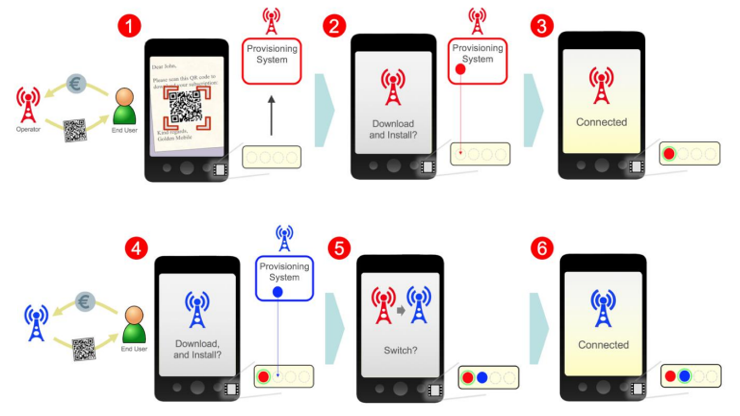
\includegraphics[width=\linewidth]{RSP-functioning.png}
\caption{Comunicazione tra end user e operatore nel contesto del Remote SIM Provisioning.}
\label{fig:RSP-functioning}
\end{figure}
\\Per quanto riguarda l'architettura interna di RSP nello specifico, esistono due soluzioni diverse \cite{GSMA-docs-new}.
\begin{enumerate}
\item \textbf{LPA embeddato nel dispositivo mobile ma non all'interno dell'eUICC (LPAd)}: oltre alla comunicazione tra l'applicazione LPA e SM-DP+, si utilizzano delle apposite interfacce anche per la comunicazione tra l'eUICC e l'applicazione LPA, come mostrato nella figura \ref{fig:RSP-LPAd} tratta da \cite{GSMA-docs-new}.
\begin{figure}
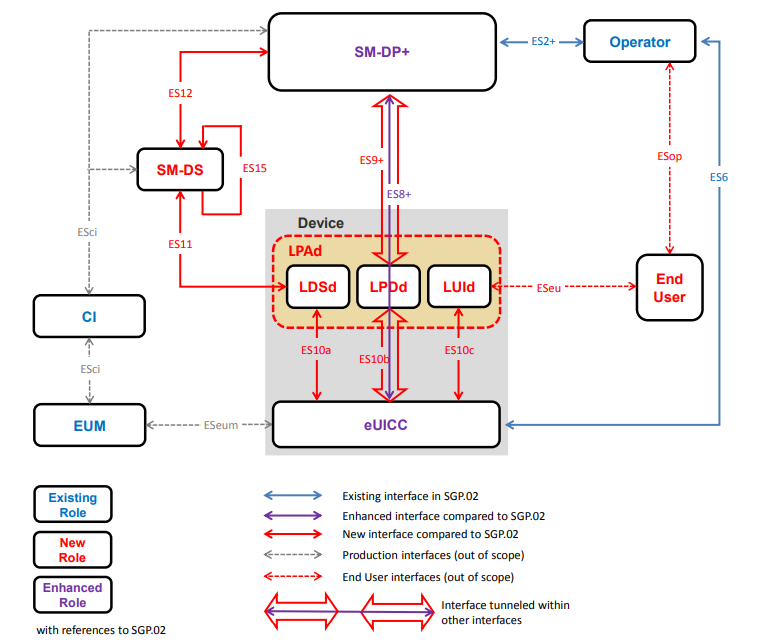
\includegraphics[width=\linewidth]{RSP-LPAd.png}
\caption{Architettura di RSP nel caso di LPA non embeddato nell'eUICC.}
\label{fig:RSP-LPAd}
\end{figure}
Di seguito è riportato un breve glossario che chiarisce il significato di alcuni componenti appartenenti all'architettura di RSP raffigurata in \ref{fig:RSP-LPAd}.
\begin{itemize}
\item \textbf{CI} = Certificate Issuer: noto anche come eSIM CA RootCA, è un'entità autorizzata a rilasciare certificati digitali.
\item \textbf{Device App} = una qualunque applicazione installata nel dispositivo mobile.
\item \textbf{Enterprise} = impresa (i.e. azienda, organizzazione o entità governativa) che si iscrive ai servizi mobili che devono essere utilizzati dai dipendenti a supporto dell'impresa stessa.
\item \textbf{EUM} = eUICC Manufacturer: è il fornitore delle eUICC e del software residente (e.g. firmware, sistema operativo); svolge anche il ruolo di certificate authority subordinata al CI e rilascia certificati all'eUICC \cite{Sec-analysis}.
\item \textbf{HRI Server} = server che fornisce le High Resolution Icon, che sono icone che vengono create per essere visualizzate in alta risoluzione.
\item \textbf{LDSd} = Local Discovery Service (quando LPA non è nell'eUICC).
\item \textbf{LPDd} = Local Profile Download (quando LPA non è nell'eUICC).
\item \textbf{LUId} = Local User Interface (quando LPA non è nell'eUICC).
\item \textbf{SM-DS} = Subscription Manager Discovery Server: è il componente che fornisce un mezzo a SM-DP+ per raggiungere l'eUICC senza dover sapere a quale rete il dispositivo è connesso.
\end{itemize}
\item \textbf{LPA embeddato all'interno dell'eUICC (LPAe)}: sono necessarie solo delle interfacce tra l'eUICC e SM-DP+, come mostrato nella figura \ref{fig:RSP-LPAe} tratta da \cite{GSMA-docs-new}.
\begin{figure}
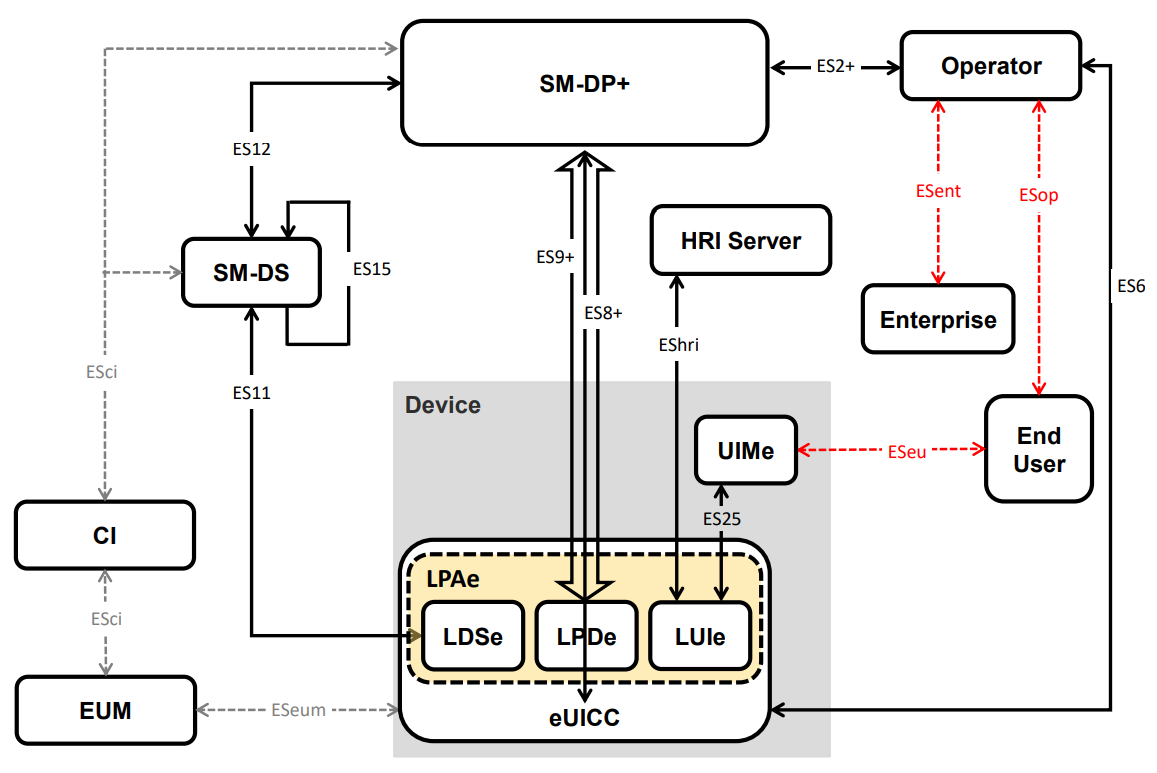
\includegraphics[width=\linewidth]{RSP-LPAe.png}
\caption{Architettura di RSP nel caso di LPA embeddato nell'eUICC.}
\label{fig:RSP-LPAe}
\end{figure}
Successivamente è riportato un breve glossario che chiarisce il significato di alcuni componenti appartenenti all'architettura di RSP raffigurata in \ref{fig:RSP-LPAe}.
\begin{itemize}
\item \textbf{LDSe} = Local Discovery Service (quando LPA è nell'eUICC).
\item \textbf{LPDe} = Local Profile Download (quando LPA è nell'eUICC).
\item \textbf{LUIe} = Local User Interface (quando LPA è nell'eUICC).
\item \textbf{UIMe} = User Inteface Module.
\end{itemize}
\end{enumerate}

\subsection{Interfacce presenti nell'architettura di RSP}
Sono illustrate nella tabella \ref{tab:interfaces}, costruita a partire da informazioni tratte da \cite{GSMA-docs-new}.\\
\begin{table}[h!]
\begin{center}
\captionsetup{skip=4pt}
\caption{Interfacce in RSP}
\label{tab:interfaces}
\begin{tabularx}{\textwidth}{|c|c|c|X|} % <-- Alignments: 1st column center, 2nd center and 3rd center, with vertical lines in between
\hline
\textbf{Interfaccia} & \textbf{Componente 1} & \textbf{Componente 2} & \textbf{Descrizione}\\
\hline
ES2+ & Operatore & SM-DP+ & Viene usata dall'operatore per invocare la preparazione del Profile Package*.\\
\hline
ES6 & Operatore & eUICC & Viene usata dall'operatore per gestire il contenuto dei profili.\\
\hline
ES8+ & SM-DP+ & eUICC & Fornisce un canale end-to-end sicuro tra SM-DP+ e l'eUICC per l'amministrazione dell'ISD-P** e del relativo profilo durante il download e l'installazione.\\
\hline
ES9+ & SM-DP+ & LPD & Viene usata per fornire trasporto sicuro tra SM-DP+ e LPD per la consegna del Profile Package.\\
\hline
ES10a & LDSd & eUICC & Viene usata da LPAd per ottenere gli indirizzi configurati dall'eUICC per Root SM-DS*** (gestione di una Discovery Request).\\
\hline
ES10b & LPDd & eUICC & Viene usata da LPAd per trasferire un Profile Package all'eUICC.\\
\hline
ES10c & LUId & eUICC & Viene usata da LPAd per la gestione locale dei profili installati sull'eUICC da parte dell'end user (e.g. Enable, Disable, Delete).\\
\hline
ES11 & LDS & SM-DS & Viene usata per l'ottenimento di eventi.\\
\hline
ES12 & SM-DP+ & SM-DS & Viene usata per la gestione degli eventi.\\
\hline
ES15 & SM-DS & SM-DS & Viene usata per connettere gli SM-DS tra loro nel caso in cui ce ne sia più di uno.\\
\hline
ES22 & LPAd & Device App & Viene usata da un'applicazione del dispositivo mobile per interoperare con l'LPA.\\
\hline
ES25 & UIMe & LUIe & Viene usata per trasferire verso l'LPA le interazioni dell'end user.\\
\hline
ESop & Operatore & End user & È specifica per le relazioni di business tra l'operatore e l'end user.\\
\hline
ESeu & End user & LUI & È specifica per le relazioni di business tra l'end user e la LUI.\\
\hline
ESeum & eUICC & EUM & È specifica per le relazioni di business tra l'eUICC e l'EUM.\\
\hline
ESci & CI & SM-DP+, SM-DS, EUM & Viene usata per richiedere certificati.\\
\hline
EShri & LUI & HRI Server & Viene usata per recuperare le High Resolution Icon.\\
\hline
ESent & Operatore & Enterprise & È un'interfaccia che prescinde dagli scopi del presente documento.\\
\hline
ESapp & Operatore & Device App & È un'interfaccia che prescinde dagli scopi del presente documento.\\
\hline
\end{tabularx}
\end{center}
\end{table}
\\\textit{*Un Profile Package è un pacchetto di dati associato a un profilo che contiene le informazioni di configurazione necessarie per attivare e utilizzare quel profilo all'interno di una scheda eSIM. Esistono diversi tipi di Profile Package: l'Unprotected Profile Package (UPP) è un pacchetto di dati non protetto da alcun meccanismo di sicurezza, come l'autenticazione o la crittografia; il Protected Profile Package (PPP) è un pacchetto di dati protetto da alcuni meccanismi di sicurezza; il Bound Profile Package (BPP) è un pacchetto di dati legato a un particolare dispositivo o a una piattaforma di servizi; il Segmented Bound Profile Package (SBPP), infine, non è altro che un BPP suddiviso in molteplici segmenti che possono essere utilizzati in modo indipendente e separato.}\\
\textit{**ISD-P (Issuer Security Domain Profile) è un contenitore sicuro che ospita un unico profilo.}\\
\textit{***Root SM-DS è il server primario utilizzato da un operatore di rete mobile per gestire le attivazioni e le disattivazioni delle sottoscrizioni e per gestire funzionalità come l'autenticazione e l'autorizzazione degli utenti. D'altra parte, si hanno gli Alternative SM-DS, che sono server di backup a cui si ricorre quando il Root SM-DS non è disponibile.}

\section{Architettura dell'eUICC}
Nella figura \ref{fig:eUICC-arch} tratta da \cite{GSMA-docs-new} è schematizzata l'architettura interna del chip eUICC, dove i riquadri e le frecce in rosso sono relativi rispettivamente ai componenti e alle interfacce che, nell'ambito dell'eUICC, sono presenti esclusivamente nel caso in cui l'applicazione LPA sia effettivamente embeddata all'interno dell'eUICC (LPAe).
\begin{figure}
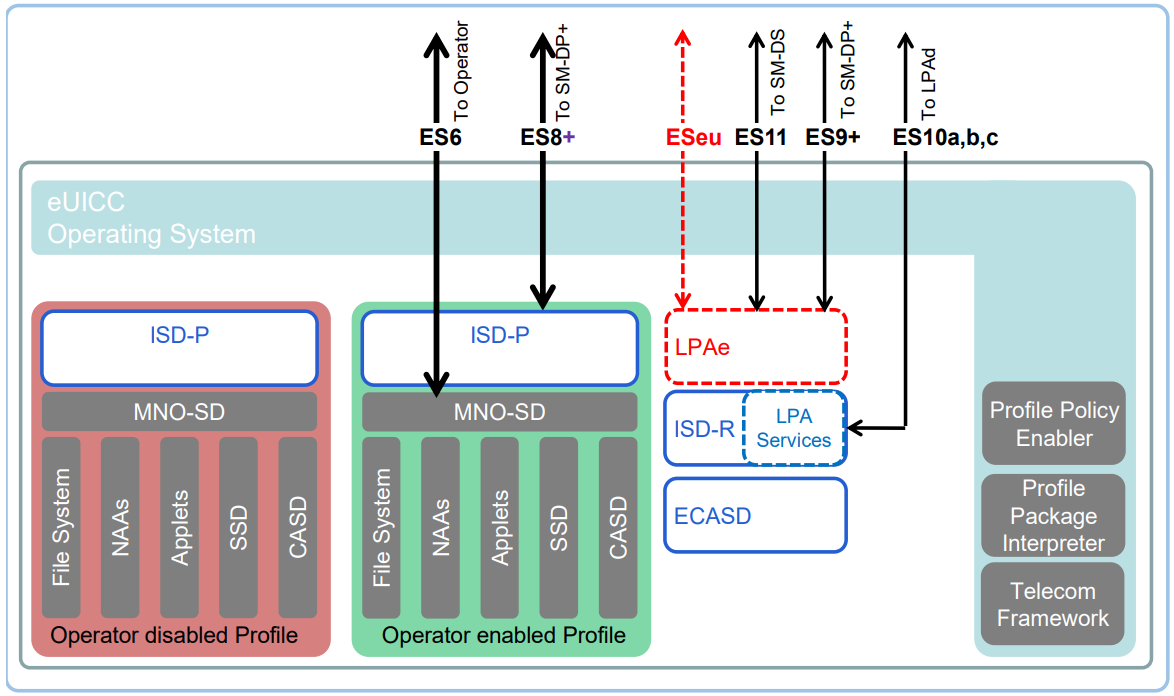
\includegraphics[width=\linewidth]{eUICC-arch.png}
\caption{Architettura dell'eUICC.}
\label{fig:eUICC-arch}
\end{figure}
\\Di seguito, invece, è riportato un breve glossario che chiarisce il significato di alcuni componenti appartenenti all'architettura dell'eUICC raffigurata in \ref{fig:eUICC-arch}.
\begin{itemize}
\item \textbf{CASD} = Controller Authority Security Domain: è un'area di storage sicura all'interno dell'ISD-P in cui vengono memorizzate le credenziali richieste per supportare le funzionalità di sicurezza sensibili.
\item \textbf{ECASD} = Embedded Controller Authority Security Domain: è il componente CASD direttamente incapsulato all'interno dell'eUICC.
\item \textbf{ISD-R} = Issuer Security Domain Root: è il componente responsabile della creazione di nuovi ISD-P e della gestione del loro ciclo di vita.
\item \textbf{LPA Services} = i seguenti quattro servizi: trasferimento del Bound Profile Package da LPAd all'ISD-P; ottenimento della lista dei profili installati; recupero dell'EID (eUICC ID); ottenimento delle operazioni di gestione del profilo locale (Local Profile Management Operations).
\item \textbf{MNO-SD} = Mobile Network Operator Security Domain: è la parte del profilo posseduta dall'operatore che fornisce all'operatore Over The Air (OTA) un canale di comunicazione sicuro; viene usato per gestire il contenuto di un profilo una volta che è stato abilitato.
\item \textbf{NAAs} = Network Access Applications: sono le applicazioni che consentono l'accesso alla rete.
\item \textbf{Profile Package Interpreter} = servizio del sistema operativo dell'eUICC che traduce i dati del Profile Package in un profilo installato all'interno dell'ISD-P codificando usando il formato interno dell'eUICC.
\item \textbf{Profile Policy Enabler} = componente che verifica che un il profilo eSIM possa essere installato sull’eUICC.
\item \textbf{SSD} = Supplementary Security Domain: è un'area di memoria protetta all'interno dell'ISD-P che viene utilizzata per l'esecuzione di funzioni di sicurezza come le operazioni crittografiche. Di fatto, il suo scopo principale è quello di proteggere le informazioni riservate dell'utente (i.e. chiavi, password) da accessi non autorizzati e attacchi esterni.
\item \textbf{Telecom Framework} = servizio del sistema operativo dell'eUICC che fornisce algoritmi di autenticazione di rete standardizzati alle applicazioni NAAs ospitate nei rispettivi ISD-P.
\end{itemize}

\subsection{Caratteristiche hardware e software dell'eUICC}
\begin{enumerate}[itemsep=0pt]
\item Deve essere resistente al tampering dei componenti hardware.
\item Contiene un unico ECASD (eUICC Controlling Authority Security Domain), che è un componente responsabile dello storage sicuro di chiavi e certificati.
\item Supporta SHA-1.
%\item Supporta TUAK, che è un particolare algoritmo crittografico di 3GPP, dove 3GPP (Third Generation Partnership Project) è il consorzio industriale che definisce gli standard per la tecnologia 5G .
\item Supporta Milenage, che è un set di funzioni di autenticazione e di generazione di chiavi.
\item Tutte le funzioni crittografiche devono essere resistenti al tampering e agli attacchi side-channel.
\end{enumerate}

\section{Chiavi crittografiche e certificati}
\subsection{Chiavi crittografiche}
I principali attori che interagiscono nel protocollo RSP sono l'eUICC, l'LPA e il server SM-DP+. Le chiavi utilizzate da loro hanno tutte un nome di tipo $<$XX$>$.$<$YY$>$.$<$ZZ$>$ \cite{GSMA-docs-new}, dove:
\begin{itemize}
\item \textbf{$<$XX$>$}: indica la natura della chiave (i.e. chiave pubblica PK, chiave privata SK, chiave pubblica one-time otPK, chiave privata one-time otSK).
\item \textbf{$<$YY$>$}: indica il proprietario della chiave.
\item \textbf{$<$ZZ$>$}: indica l'utilizzo della chiave (i.e. digital signature SIG, key agreement KA, TLS).
\end{itemize}
Le chiavi di maggiore rilievo, comunque sia, sono riportate nella tabella \ref{tab:keys} tratta da \cite{GSMA-docs-old}.
\begin{table}[h!]
\begin{center}
\captionsetup{skip=4pt}
\caption{Chiavi crittografiche in RSP}
\label{tab:keys}
\begin{tabularx}{\textwidth}{|c|X|}
\hline
\textbf{Nome} & \textbf{Descrizione}\\
\hline
PK.EUICC.SIG & Chiave pubblica dell'eUICC usata per verificare le signature dell'eUICC. È inclusa nel certificato CERT.EUICC.SIG.\\
\hline
SK.EUICC.SIG & Chiave privata dell'eUICC usata per generare le signature.\\
\hline
PK.DPauth.SIG & Chiave pubblica del server SM-DP+ usata per verificare le signature del server. È inclusa nel certificato CERT.DPauth.SIG.\\
\hline
SK.DPauth.SIG & Chiave privata del server SM-DP+ usata per generare le signature per autenticarsi all'eUICC.\\
\hline
PK.DPpb.SIG & Chiave pubblica del server SM-DP+ usata per verificare le signature del server comprese nel BPP.  È inclusa nel certificato CERT.DPpb.SIG.\\
\hline
SK.DPpb.SIG & Chiave privata del server SM-DP+ usata per generare le signature per il binding dei profili.\\
\hline
PK.DSauth.SIG & Chiave pubblica del server SM-DS usata per verificare le signature di SM-DS. È inclusa nel certificato CERT.DSauth.SIG.\\
\hline
SK.DSauth.SIG & Chiave privata del server SM-DS usata per generare le signature per autenticarsi all'eUICC.\\
\hline
PK.EUM.SIG & Chiave pubblica dell'EUM usata per verificare i certificati degli eUICC. È inclusa nel certificato CERT.EUM.SIG.\\
\hline
SK.EUM.SIG & Chiave privata dell'EUM usata per firmare i certificati degli eUICC.\\
\hline
PK.CI.SIG &  Chiave pubblica del CI usata per verificare i certificati dell'EUM dei server SM-DS e del server SM-DP+.\\
\hline
SK.CI.SIG & Chiave privata del CI usata per firmare i certificati dell'EUM dei server SM-DS e del server SM-DP+.\\
\hline
otPK.EUICC.KA & Chiave pubblica one-time dell'eUICC usata per il key agreement.\\
\hline
otSK.EUICC.KA & Chiave privata one-time dell'eUICC usata per il key agreement.\\
\hline
otPK.DP.KA & Chiave pubblica one-time del server SM-DP+ usata per il key agreement.\\
\hline
otSK.DP.KA & Chiave privata one-time del server SM-DP+ usata per il key agreement.\\
\hline
PK.DP.TLS & Chiave pubblica del server SM-DP+ usata per verificare le signature TLS del server. È inclusa nel certificato CERT.DP.TLS.\\
\hline
SK.DP.TLS & Chiave privata del server SM-DP+ usata per generare le signature per autenticarsi all'LPA.\\
\hline
PK.DS.TLS & Chiave pubblica del server SM-DS usata per verificare le signature TLS di SM-DS. È inclusa nel certificato CERT.DS.TLS.\\
\hline
SK.DS.TLS & Chiave privata del server SM-DS usata per generare le signature per autenticarsi all'LPA.\\
\hline
\end{tabularx}
\end{center}
\end{table}

\subsection{Certificati}
I certificati propri dei principali componenti che partecipano all'interazione data dal protocollo RSP sono riportati nella tabella \ref{tab:cert} tratta da \cite{GSMA-docs-new}.\\
\begin{table}[h!]
\begin{center}
\captionsetup{skip=4pt}
\caption{Certificati in RSP}
\label{tab:cert}
\begin{tabularx}{\textwidth}{|c|X|X|}
\hline
\textbf{Nome} & \textbf{Descrizione} & \textbf{Note}\\
\hline
CERT.CI.SIG & Certificato GSMA CI & Viene firmato e rilasciato da se stesso.\\
\hline
CERT.CISubCA.SIG & Certificato GSMA CI subordinato & Se esistente, viene firmato e rilasciato dal CI root.\\
\hline
CERT.EUM.SIG & Certificato EUM & Viene firmato e rilasciato dal CI (root o subordinato).\\
\hline
CERT.EUMSubCA.SIG & Certificato EUM subordinato & Se esistente, viene firmato e rilasciato dall'EUM root.\\
\hline
CERT.DPSubCA.SIG & Certificato SM-DP+ intermediario & Viene firmato e rilasciato dal CI (root o subordinato).\\
\hline
CERT.DPauth.SIG & Certificato SM-DP+ per autenticarsi all'eUICC & Viene firmato e rilasciato dal SM-DP+ intermediario o dal CI (root o subordinato).\\
\hline
CERT.DPpb.SIG & Certificato SM-DP+ per rilasciare e firmare i profili eSIM & Viene firmato e rilasciato dal SM-DP+ intermediario o dal CI (root o subordinato).\\
\hline
CERT.DP.TLS & Certificato TLS di SM-DP+ & Viene firmato e rilasciato dal SM-DP+ intermediario o dal CI (root o subordinato).\\
\hline
CERT.DSSubCA.SIG & Certificato SM-DS intermediario & Viene firmato e rilasciato dal CI (root o subordinato).\\
\hline
CERT.DSauth.SIG & Certificato SM-DS & Viene firmato e rilasciato dal SM-DS intermediario o dal CI (root o subordinato).\\
\hline
CERT.DS.TLS & Certificato TLS di SM-DS & Viene firmato e rilasciato dal SM-DS intermediario o dal CI (root o subordinato).\\
\hline
CERT.EUICC.SIG & Certificato eUICC & Viene firmato e rilasciato dall'EUM (root o subordinato).\\
\hline
CERT.CA.SIG & Certificato di una qualunque CA pubblica & Può firmare e rilasciare certificati TLS.\\
\hline
\end{tabularx}
\end{center}
\end{table}
\\La figura \ref{fig:cert-chain} tratta da \cite{GSMA-docs-old} definisce uno schema riassuntivo della struttura originale della catena di certificati definita dalla Public Key Infrastructure (PKI) di RSP.\\
Attualmente, invece, la struttura della certificate chain è più complessa e introduce molteplici varianti differenti (i.e. presenza o meno di GSMA CI subordinati, presenza o meno di EUM subordinati, presenza o meno di SM-DP+ intermediari, presenza o meno di SM-DS intermediari). Di seguito, per semplicità, più porzioni distinte della catena verranno analizzate separatamente.
\begin{itemize}
\item Porzione della catena comprendente il CI, l'EUM e l'eUICC: è riportata nella figura \ref{fig:cert-chain-new1} tratta da \cite{GSMA-docs-new} e prevede quattro varianti differenti.
\begin{itemize}
\item \textbf{Variante O (originale)}: il CI root rilascia certificati per l'EUM root, il quale rilascia a sua volta certificati per l'eUICC.
\item \textbf{Variante A}: il CI root rilascia certificati per l'EUM root; l'EUM root rilascia certificati per l'EUM subordinato; l'EUM subordinato, infine, rilascia certificati per l'eUICC.
\item \textbf{Variante B}: il CI root rilascia certificati per il CI subordinato; il CI subordinato rilascia certificati per l'EUM root; l'EUM root, infine, rilascia certificati per l'eUICC.
\item \textbf{Variante C}: il CI root rilascia certificati per il CI subordinato; il CI subordinato rilascia certificati per l'EUM root; l'EUM root rilascia certificati per l'EUM subordinato; l'EUM subordinato, infine, rilascia certificati per l'eUICC.
\end{itemize}
\item Porzione della catena comprendente il CI e i certificati di tipo SIG di SM-DP+ e SM-DS: è riportata nella figura \ref{fig:cert-chain-new2} tratta da \cite{GSMA-docs-new} e prevede quattro varianti differenti.
\begin{itemize}
\item \textbf{Variante O (originale)}: il CI root rilascia direttamente i certificati CERT.DPauth.SIG, CERT.DPpb.SIG, CERT.DSauth.SIG.
\item \textbf{Variante A}: il CI root rilascia certificati per l'SM-DP+ intermediario e l'SM-DS intermediario; l'SM-DP+ intermediario rilascia i certificati  CERT.DPauth.SIG, CERT.DPpb.SIG; l'SM-DS intermediario rilascia il certificato CERT.DSauth.SIG.
\item \textbf{Variante B}: il CI root rilascia certificati per il CI subordinato, il quale rilascia a sua volta i certificati CERT.DPauth.SIG, CERT.DPpb.SIG, CERT.DSauth.SIG.
\item \textbf{Variante C}: il CI root rilascia certificati per il CI subordinato; il CI subordinato rilascia certificati per l'SM-DP+ intermediario e l'SM-DS intermediario; l'SM-DP+ intermediario rilascia i certificati CERT.DPauth.SIG, CERT.DPpb.SIG; l'SM-DS intermediario rilascia il certificato CERT.DSauth.SIG.
\end{itemize}
\item Porzione della catena comprendente il CI e i certificati TLS di SM-DP+ e SM-DS: è riportata nella figura \ref{fig:cert-chain-new3} tratta da \cite{GSMA-docs-new} e prevede quattro varianti differenti.
\begin{itemize}
\item \textbf{Variante O (originale)}: il CI root rilascia direttamente i certificati CERT.DP.TLS, CERT.DS.TLS.
\item \textbf{Variante A}: il CI root rilascia i certificati per l'SM-DP+ intermediario e l'SM-DS intermediario; l'SM-DP+ intermediario rilascia il certificato CERT.DP.TLS; l'SM-DS intermediario rilascia il certificato CERT.DS.TLS.
\item \textbf{Variante B}: il CI root rilascia certificati per il CI subordinato, il quale rilascia a sua volta i certificati CERT.DP.TLS, CERT.DS.TLS.
\item \textbf{Variante C}: il CI root rilascia certificati per il CI subordinato; il CI subordinato rilascia certificati per l'SM-DP+ intermediario e l'SM-DS intermediario; l'SM-DP+ intermediario rilascia il certificato CERT.DP.TLS; l'SM-DS intermediario rilascia il certificato CERT.DS.TLS.
\end{itemize}
\end{itemize}
Per quanto riguarda i certificati TLS, al posto del CI, può esserci come root qualunque CA pubblica, come mostrato nella figura \ref{fig:cert-chain-new4} tratta da \cite{GSMA-docs-new}. Anche con questa soluzione esistono diverse varianti.
\begin{itemize}
\item \textbf{Prima variante OO (originale)}: la CA pubblica root rilascia direttamente i certificati CERT.DP.TLS, CERT.DS.TLS.
\item \textbf{Seconda variante OO}: la CA pubblica root rilascia certificati per la CA pubblica subordinata, la quale rilascia a sua volta i certificati CERT.DP.TLS, CERT.DS.TLS.
\item \textbf{Prima variante AA}: la CA pubblica rilascia certificati per l'SM-DP+ intermediario e l'SM-DS intermediario; l'SM-DP+ intermediario rilascia il certificato CERT.DP.TLS; l'SM-DS intermediario rilascia il certificato CERT.DS.TLS.
\item \textbf{Seconda variante AA}: la CA pubblica rilascia certificati per la CA pubblica subordinata; la CA pubblica subordinata rilascia certificati per l'SM-DP+ intermediario e l'SM-DS intermediario; l'SM-DP+ intermediario rilascia il certificato CERT.DP.TLS; l'SM-DS intermediario rilascia il certificato CERT.DS.TLS.
\end{itemize}
\begin{figure}
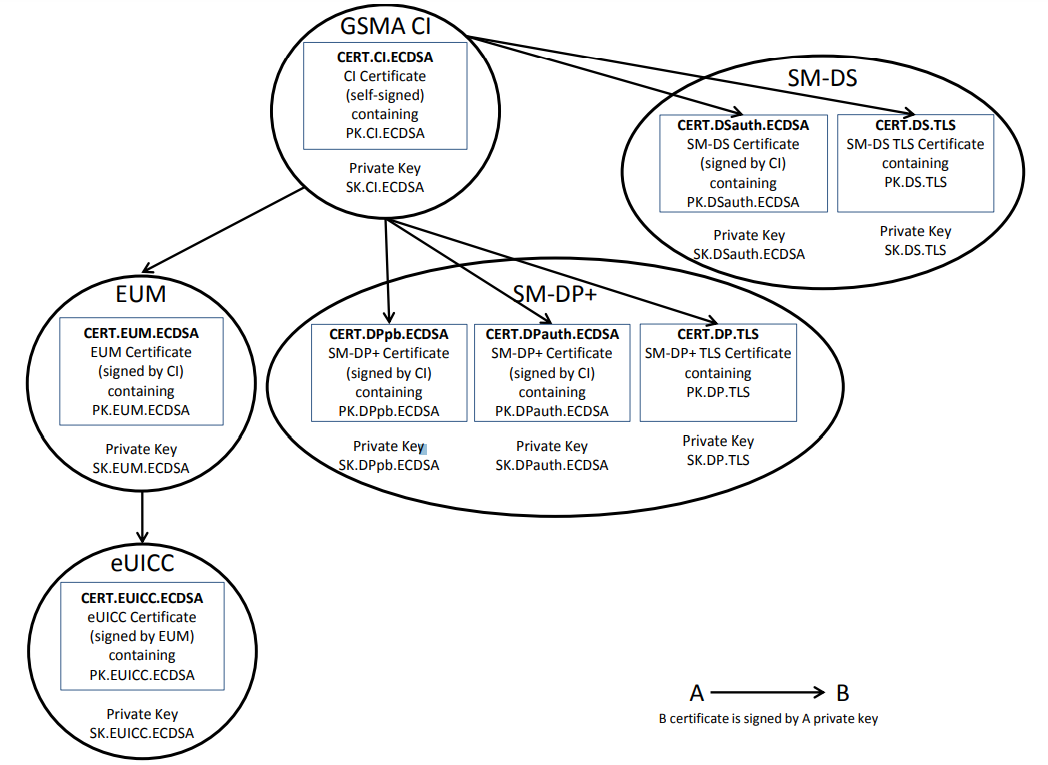
\includegraphics[width=\linewidth]{cert-chain.png}
\caption{Catena di certificati definita originariamente dalla PKI di RSP.}
\label{fig:cert-chain}
\end{figure}
\begin{figure}
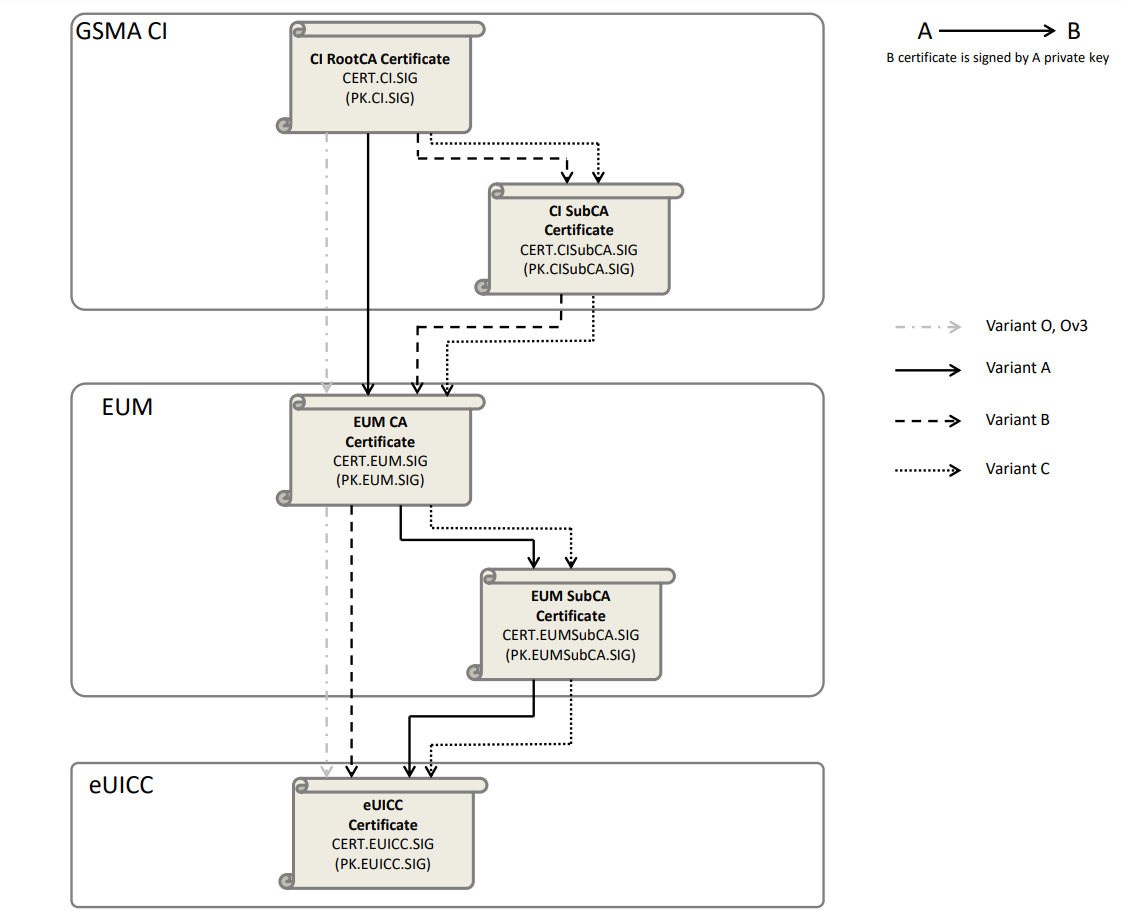
\includegraphics[width=\linewidth]{cert-chain-new1.png}
\caption{Prima porzione dell'attuale catena di certificati definita dalla PKI di RSP.}
\label{fig:cert-chain-new1}
\end{figure}
\begin{figure}
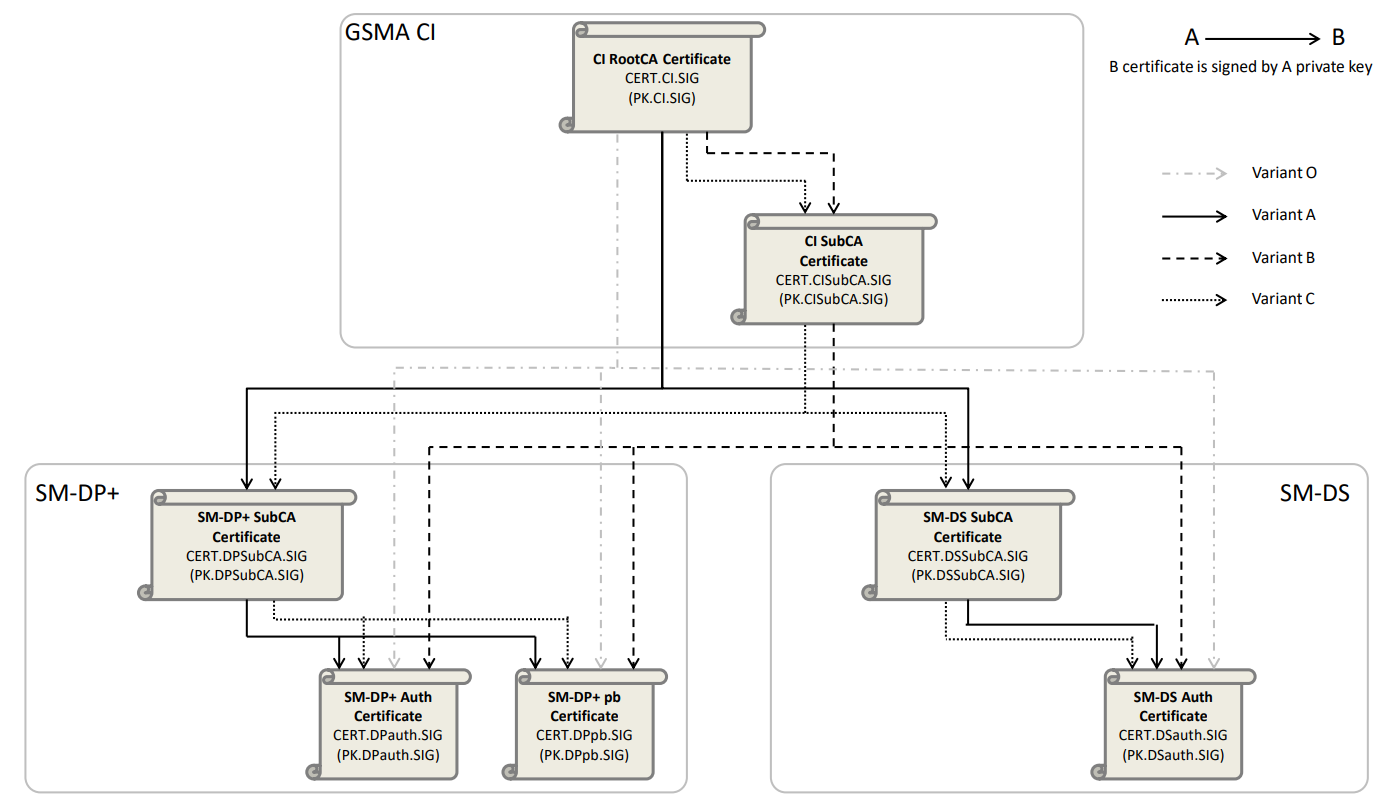
\includegraphics[width=\linewidth]{cert-chain-new2.png}
\caption{Prima porzione dell'attuale catena di certificati definita dalla PKI di RSP.}
\label{fig:cert-chain-new2}
\end{figure}
\begin{figure}
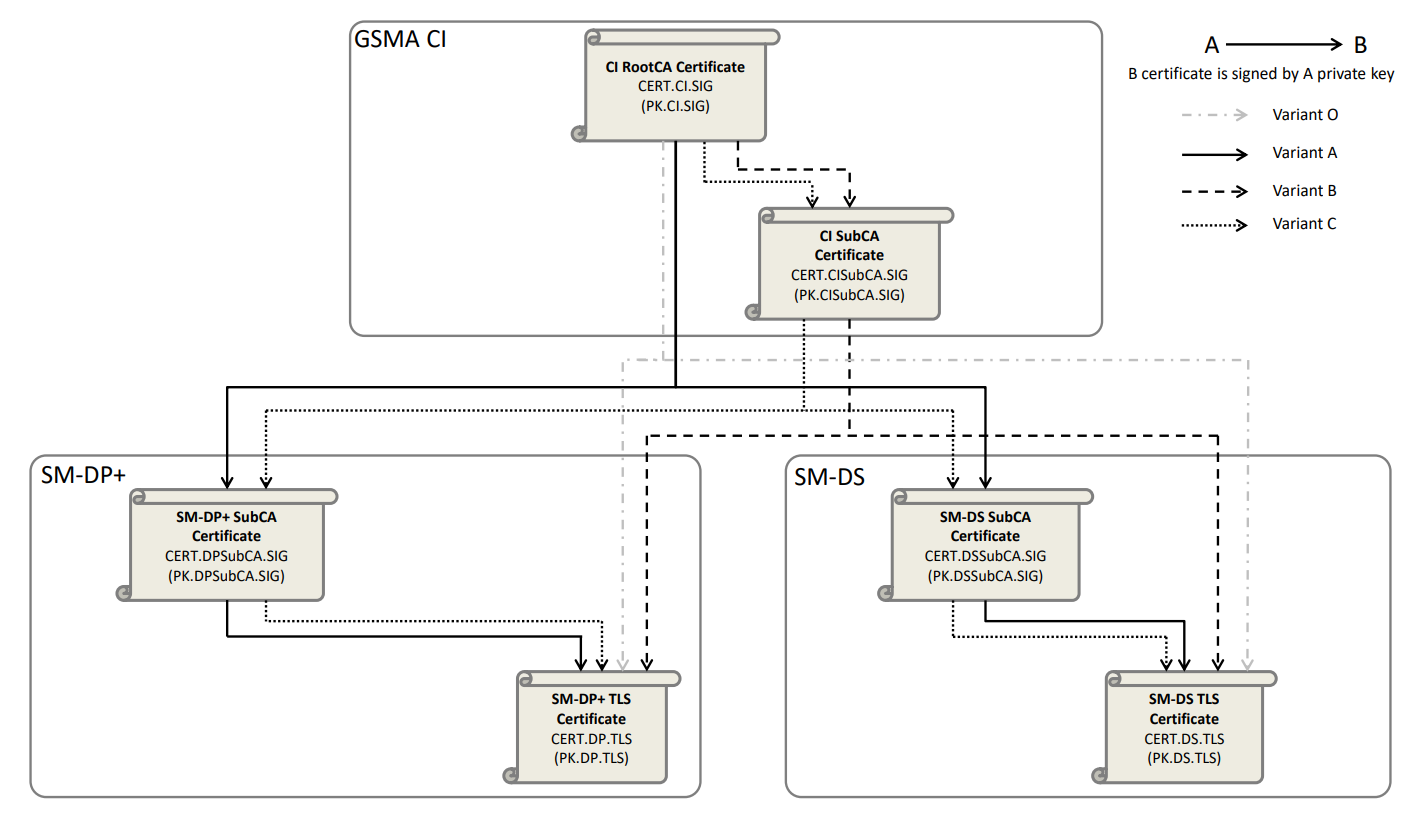
\includegraphics[width=\linewidth]{cert-chain-new3.png}
\caption{Prima porzione dell'attuale catena di certificati definita dalla PKI di RSP.}
\label{fig:cert-chain-new3}
\end{figure}
\begin{figure}
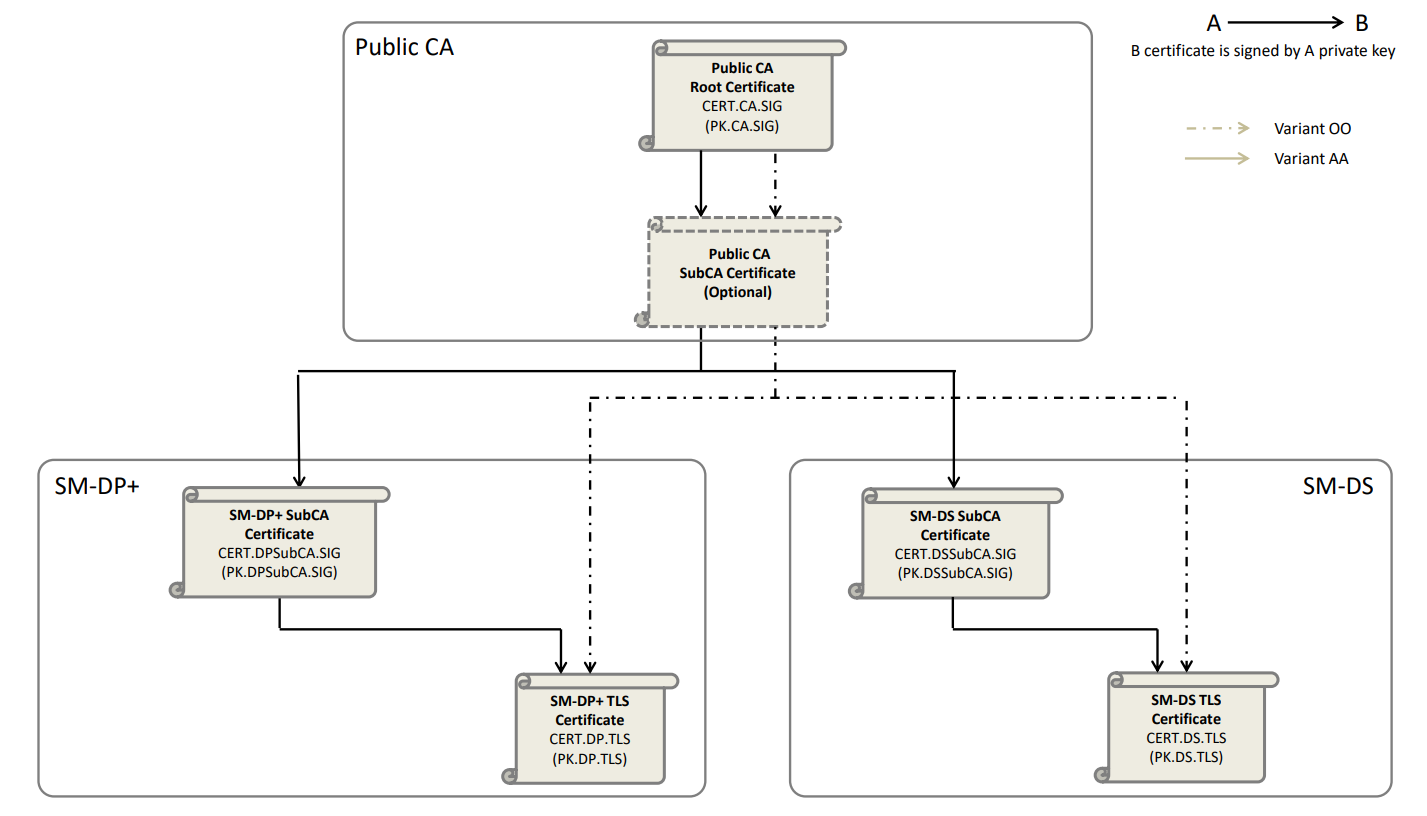
\includegraphics[width=\linewidth]{cert-chain-new4.png}
\caption{Prima porzione dell'attuale catena di certificati definita dalla PKI di RSP.}
\label{fig:cert-chain-new4}
\end{figure}
All'interno della PKI, il Certificate Issuer di GSMA (CI) è la Root Certification Authority del servizio RSP e, di conseguenza, rappresenta il nodo radice della catena. Inoltre, tutti i certificati possono essere rilasciati direttamente dal CI (root o subordinato), fatta eccezione di CERT.EUICC.SIG che, invece, viene rilasciato dall'EUM (root o subordinato). Tutti i certificati che possono essere rilasciati direttamente dal CI hanno la possibilità di essere revocati in qualunque momento, in particolar modo se le entità corrispondenti (CI, EUM, SM-DP+, SM-DS) vengono compromesse. D'altra parte, i certificati eUICC (CERT.EUICC.SIG) non vengono revocati in modo individuale: di fatto, è difficile che un singolo eUICC venga compromesso. Piuttosto, è più verosimile che un modello eUICC o un intero batch di produzione di eUICC venga dichiarato come compromesso; quando ciò avviene, quello che si fa è revocare direttamente il certificato EUM (CERT.EUM.SIG) associato a quel modello o batch di produzione di eUICC \cite{GSMA-docs-new}.\\
Il CI fornisce una Certificate Revocation List (CRL), che è la lista dei certificati revocati tra tutti i certificati non scaduti che erano stati rilasciati da quello stesso CI. Ciascun CI, per giunta, deve pubblicare la propria CRL sia periodicamente, sia ogni volta che viene revocato un particolare certificato \cite{GSMA-docs-new}.\\
In realtà, i certificati relativi alla PKI di RSP di cui si è discusso finora non sono gli unici certificati utilizzati per effettuare il deployment dei profili eSIM: esiste anche un certificato per firmare l'applicazione LPA e un certificato da inserire in ciascun profilo eSIM da distribuire all'end user. Dove entrano in gioco tali certificati? Con riferimento alla guida di Android per le API e per l'implementazione del deployment dei profili eSIM \cite{Android-docs}, l'interazione tra un'applicazione LPA e l'interfaccia all'eUICC (legata al componente EuiccManager in \cite{Android-docs}) può avvenire solo se l'applicazione dispone dei privilegi dell'operatore. Di norma, tali privilegi sono conferiti all'applicazione se il certificato usato per firmarla coincide col certificato presente nel profilo fornito da SM-DP+.

\section{Interazione tra eUICC, LPA, SM-DP+ e operatore}
\subsection{Sicurezza TLS}
Il protocollo TLS, la cui versione 1.2 è definita in RFC 5246 \cite{RFC-5246} e la cui versione 1.3 è definita in RFC 8446 \cite{RFC-8446}, è utilizzato per proteggere il traffico sulle interfacce ES2+ (tra server SM-DP+ e operatore) e ES9+ (tra server SM-DP+ e LPA). In particolare, in ES2+ è prevista la mutua autenticazione tra le parti, mentre in ES9+ è prevista solo l'autenticazione del server. La documentazione di GSMA di riferimento \cite{GSMA-docs-new} sottolinea l'obbligatorietà di fare uso di TLS v1.2 sia per gli algoritmi di autenticazione e autorizzazione, sia per l'integrità dei messaggi, sia per la confidenzialità. In realtà, introduce anche la possibilità (e suggerisce) di utilizzare TLS v1.3, che è la versione più recente di TLS e risolve le vulnerabilità che caratterizzano TLS v1.2, per cui, in linea di principio, dovrebbe risultare particolarmente difficoltoso da penetrare. Tuttavia, attualmente sembra essere solo un suggerimento, per cui nei capitoli successivi potrebbe essere necessario verificare a livello pratico qual è la versione di TLS utilizzata per proteggere la comunicazione tra LPA e server SM-DP+.\\
Un discorso analogo vale per l'interazione che si ha nella mutua autenticazione tra l'eUICC e il server SM-DP+, dove le due parti interagiscono tra loro tramite un TLS tunnel \cite{Sec-analysis}. Per quanto invece riguarda la comunicazione tra eUICC e applicazione LPA, è richiesto l'utilizzo di un pairwise secure channel (ovvero di un canale di comunicazione sicuro rispetto alla confidenzialità e all'autenticazione dei messaggi) che collega le due parti all'interno del dispositivo mobile \cite{Sec-analysis}. Tuttavia, non esiste una specifica universale che imponga l'utilizzo di un particolare protocollo di crittografia per proteggere il pairwise secure channel; il protocollo più utilizzato a tal proposito rimane TLS ma, di nuovo, potrebbe essere necessario stabilire con un approccio pratico se nel canale di comunicazione tra eUICC e LPA viene utilizzato TLS oppure un protocollo differente.

\subsection{Regole per la comunicazione in RSP}
Qualunque comunicazione remota definita per RSP deve far fede alle regole riportate di seguito \cite{GSMA-docs-new}.
\begin{itemize}
\item \textbf{Mutua autenticazione tra eUICC e server SM-DP+}: il server deve essere autenticato per primo da parte dell'eUICC, dove il processo di autenticazione deve includere la verifica di una catena di certificati del server. D'altra parte, l'eUICC deve essere autenticato in un secondo momento da parte del server, dove il processo di autenticazione, di nuovo, deve includere la verifica di una catena di certificati dell'eUICC; l'autenticazione dell'eUICC non si applica all'applicazione LPA.
\item \textbf{Privacy dei dati}: l'eUICC, in quanto client, non deve rivelare alcuna informazione privata a un server SM-DP+ non autenticato. Inoltre, non deve generare materiale firmato prima del completamento del processo di autenticazione del server.
\item \textbf{Protezione della comunicazione}: quando possibile, la comunicazione tra eUICC e server SM-DP+, oltre a essere protetta dall'integrità dei messaggi, dalla cifratura e dall'autenticazione del mittente, dovrebbe essere caratterizzata dalla proprietà di Perfect Forward Secrecy. Secondo tale proprietà, se anche una chiave a lungo termine viene compromessa, le chiavi di sessione generate a partire da essa rimangono comunque riservate.
\item \textbf{Autorizzazione}: il server SM-DP+ deve sempre verificare che il client che ha inviato una richiesta sia effettivamente autorizzato prima di far partire l'esecuzione della funzione desiderata.
\end{itemize}

\subsection{Step dell'interazione in RSP}
L'interazione tra le parti, nel contesto del protocollo RSP, avviene in quattro fasi distinte: profile ordering, download initialization, common handshake e profile download \cite{Sec-analysis}.
\begin{itemize}
\item \textbf{Profile ordering \& download initialization}: nella prima fase, l'operatore richiede al server SM-DP+ di preparare un profilo eSIM, e il server gli restituisce dei download initialization pointer (che possono essere rappresentati ad esempio da un codice di attivazione). Nella seconda fase, invece, l'operatore consegna i download initialization pointer all'LPA in modo tale che poi sia possibile effettuare il download vero e proprio del profilo. Per questi primi due step, si possono seguire tre tipi di approcci differenti:
\begin{enumerate}
\item \underline{Default server approach}: la figura \ref{fig:default-server} tratta da \cite{Sec-analysis} mostra questo approccio. L'operatore (indicato con MNO - Mobile Network Operator) pre-condivide con l'eUICC l'indirizzo S del server. Quando vuole effettuare una nuova sottoscrizione e ottenere così un nuovo profilo, l'end user contatta l'operatore (messaggio 0), il quale ordina al server SM-DP+ il profilo per l'identificatore U dell'eUICC target (messaggio 1). Il server crea il nuovo profilo e lo invia all'operatore (messaggio 2), il quale notifica l'utente (messaggio 3). A tal punto, l'applicazione LPA viene avviata e, tramite un'operazione di get, recupera S dall'eUICC.
\item \underline{Activation code approach}: la figura \ref{fig:activation-code} tratta da \cite{Sec-analysis} mostra questo secondo approccio. L'operatore ordina al server SM-DP+ dei profili (messaggio 1), e il server li rende disponibili con un codice di attivazione (tipicamente un codice QR) e li restituisce all'operatore (messaggio 2). Il codice di attivazione include l'indirizzo S del server, l'identificatore $I_{ac}$ del profilo e, opzionalmente, l'OID, ovvero l'identificatore del server SM-DP+. Quando l'end user vuole effettuare una nuova sottoscrizione e ottenere così un nuovo profilo, contatta l'operatore (messaggio 0, che può essere inviato sia prima che dopo l'interazione tra operatore e SM-DP+ server appena descritta), il quale restituisce il codice di attivazione opportuno (messaggio 3).
\item \underline{SM-DS assisted approach}: è un approccio analogo all'activation code, con la differenza che SM-DP+ si appoggia sui server SM-DS per comunicare con l'eUICC.
\end{enumerate}
\item \textbf{Common handshake}: questa fase, nota anche come Common Mutual Authentication, coinvolge tre attori fondamentali: il server SM-DP+, l'applicazione LPA e l'eUICC. I relativi dettagli sono riportati nella sezione \ref{sec:mutual-auth}.
\item \textbf{Profile download}: quest'ultima fase non è altro che una continuazione della common handshake. Viene calcolato uno shared secret da cui, mediante una key derivation function (KDF), saranno derivate le chiavi di sessione k (per la cifratura) e k' (per l'integrità dei dati). Nel frattempo, avviene il download del profilo eSIM, in cui il server SM-DP+ invia all'LPA il profilo cifrato con la chiave k e l'identificatore dell'operatore di riferimento, dove entrambe le informazioni sono firmate singolarmente con la chiave k' mediante il meccanismo di message authentication code (MAC). Dopodiché, l'LPA mostra l'identificatore dell'operatore all'utente, che dovrà stabilire se fa riferimento all'operatore giusto: se sì, l'LPA inoltra tutte le informazioni all'eUICC il quale, dopo aver derivato a sua volta le chiavi di sessione k, k', dovrà decriptare il profilo P, che risulterà finalmente essere utilizzabile.
\end{itemize}
\begin{figure}
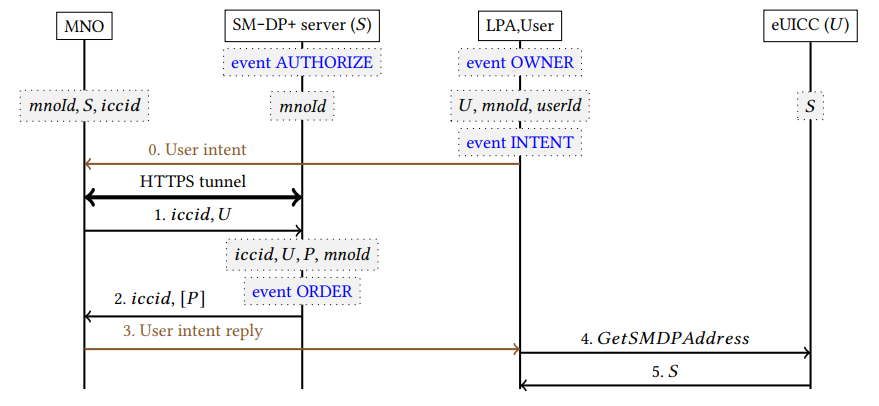
\includegraphics[width=\linewidth]{default-server.png}
\caption{Approccio default server per le fasi di profile ordering e download initialization.}
\label{fig:default-server}
\end{figure}
\begin{figure}
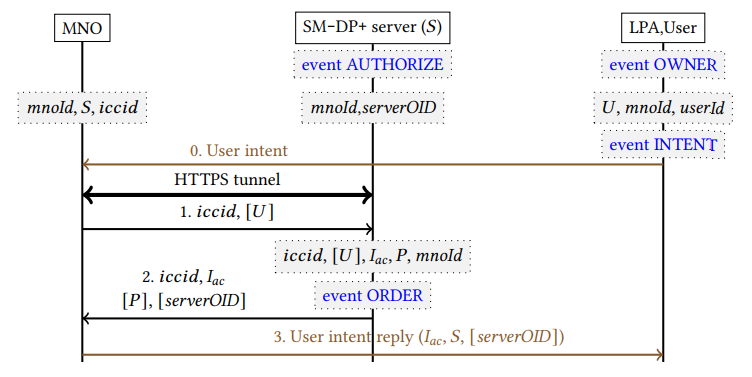
\includegraphics[width=\linewidth]{activation-code.png}
\caption{Approccio activation code per le fasi di profile ordering e download initialization.}
\label{fig:activation-code}
\end{figure}

\section{Dettagli sulla Common Mutual Authentication}\label{sec:mutual-auth}
La figura \ref{fig:common-mutual-auth} ripresa da \cite{GSMA-docs-new} illustra tutti i messaggi che il server SM-DP+, l'LPA e l'eUICC si scambiano tra loro e le operazioni che queste tre entità svolgono durante la procedura di Common Mutual Authentication. Tutti i relativi dettagli \cite{GSMA-docs-new} sono spiegati nelle sottosezioni successive. Si osservi che l'intero meccanismo resta valido e invariato se si ha un server SM-DS al posto del server SM-DP+.
\begin{figure}
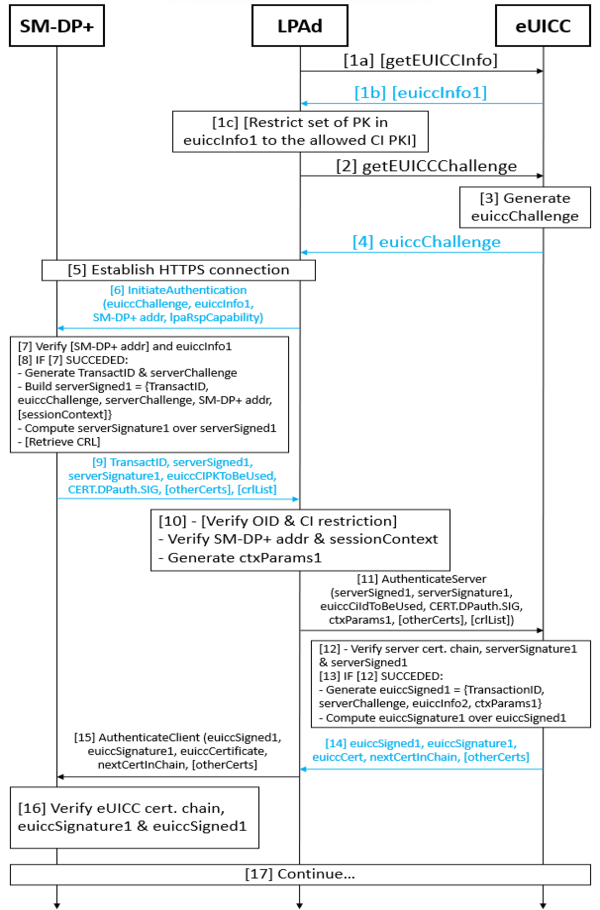
\includegraphics[width=\linewidth]{common-mutual-auth.png}
\caption{Sequence diagram che descrive la Common Mutual Authentication.}
\label{fig:common-mutual-auth}
\end{figure}

\subsection{Condizioni iniziali}
\begin{itemize}
\item Il server SM-DP+ è dotato di:
\begin{itemize}[itemsep=0pt]
\item certificato CERT.DPauth.SIG;
\item chiave privata SK.DPauth.SIG;
\item certificato del CI (CERT.CI.SIG);
\item certificato TLS CERT.DP.TLS;
\item chiave privata TLS SK.DP.TLS;
\item certificati di SM-DP+ intermediari, se esistenti (CERT.DPSubCA.SIG).
\end{itemize}
\item L'eUICC, d'altra parte, è dotato di:
\begin{itemize}[itemsep=0pt]
\item certificato CERT.EUICC.SIG;
\item chiave privata SK.EUICC.SIG;
\item certificato dell'EUM (CERT.EUN.SIG);
\item certificati di CI subordinati, se esistenti (CERT.CISubCA.SIG);
\item certificati di EUM subordinati, se esistenti (CERT.EUMSubCA.SIG);
\item chiave pubblica del CI (PK.CI.SIG).
\end{itemize}
\end{itemize}

\subsection{Procedimento}
\begin{enumerate}
\item Il primo step, che è opzionale, si articola in tre punti:
\begin{enumerate}[label=\alph*)]
\item Se non lo aveva già fatto in un momento precedente, l'LPA richiede le informazioni dell'eUICC (e.g. Specification Version Number, versione del firmware, quantità di memoria non volatile disponibile, capability dell'eUICC, categoria dell'eUICC) identificate dalla variabile euiccInfo1.
\item L'eUICC restituisce euiccInfo1 all'LPA.
\item Se esiste una restrizione sulle chiavi pubbliche dei CI consentite, l'LPA crea una nuova istanza di euiccInfo1 senza le chiavi pubbliche dei CI non compatibili. Se dopo questa operazione rimane una lista vuota di chiavi pubbliche, l'LPA informa l'end user che la procedura di mutua autenticazione deve terminare.
\end{enumerate}
\item L'LPA richiede all'eUICC una challenge (euiccChallenge).
\item L'eUICC genera la challenge che successivamente dovrà essere firmata dal server SM-DP+ per l'autenticazione del server stesso.
\item L'eUICC restituisce la challenge all'LPA.
\item L'LPA stabilisce una nuova connessione HTTPS col server SM-DP+. Il setup della sessione TLS, poiché non può riutilizzare le chiavi da una sessione precedente, deve prevedere un nuovo key exchange, che avviene nella fase del TLS handshake. Qui il server fornisce all'LPA un certificato CERT.DP.TLS e l'LPA deve verificarne la validità; se l'LPA non riesce a effettuare la verifica, il server deve inviargli un certificato CERT.DP.TLS differente, e così via, fin tanto che l'LPA non sarà riuscito a validare un certificato oppure il numero di tentativi per ritrasmettere il certificato non avrà raggiunto il limite massimo. In questo secondo caso l'LPA interrompe la procedura di Common Mutual Authentication.
\item L'LPA invoca la funzione \textit{InitiateAuthentication} passandovi come parametri le proprie capability, euiccChallenge, euiccInfo1 e l'indirizzo SM-DP+, il quale viene usato dall'LPA per accedere al server.
\item Il server SM-DP+ esegue le seguenti operazioni:
\begin{itemize}[itemsep=0pt]
\item Verificare che l'indirizzo SM-DP+ inviato dall'LPA sia valido.
\item Verificare il contenuto della variabile euiccInfo1, incluse le chiavi pubbliche del CI, tra cui deve essercene almeno una che può essere accettata dal server stesso.
\end{itemize}
Se anche solo uno di questi controlli non va a buon fine, il server restituisce una condizione di errore e l'LPA interrompe la procedura di Common Mutual Authentication.
\item Il server SM-DP+ esegue le seguenti altre operazioni:
\begin{itemize}[itemsep=0pt]
\item Generare un ID di transazione che serve per identificare la sessione RSP.
\item Generare una challenge (serverChallenge) che dovrà essere firmata dall'eUICC per l'autenticazione dell'eUICC stesso.
\item Generare una struttura dati serverSigned1 a partire dall'ID di transazione, da euiccChallenge, da serverChallenge, dall'indirizzo SM-DP+ e dal contesto di sessione.
\item Calcolare la serverSignature1 a partire da serverSigned1, utilizzando la chiave privata SK.DPauth.SIG.
\item Se sia l'eUICC che l'LPA prevedono il crlStaplingV3Support, che è la funzionalità che permette al server di fornire una Certificate Revocation List (CRL), il server deve anche recuperare la CRL per ciascun certificato che abbia l'extension set CRLDistributionPoints, che è un tipo di certificato che dà informazioni su dove è possibile ottenere una CRL.
\end{itemize}
\item Il server SM-DP+ restituisce all'LPA alcune informazioni, tra cui l'ID della transazione, serverSigned1, serverSignature1, euiccCIPKToBeUsed (che dovrà corrispondere al certificato root della certificate chain che l'eUICC dovrà comunicare), il certificato CERT.DPauth.SIG, eventuali altri certificati ed eventualmente la CRL.
\item L'LPA esegue le seguenti operazioni:
\begin{itemize}[itemsep=0pt]
\item Verificare l'OID, che è l'Object Identifier del server SM-DP+.
\item Verificare che l'indirizzo SM-DP+ restituito dal server matchi con l'indirizzo SM-DP+ che l'LPA aveva inviato allo step (6).
\item Verificare che la chiave pubblica associata al certificato CERT.DPauth.SIG sia inclusa in euiccInfo1.
\item Effettuare altre verifiche sui certificati che non verranno approfondite in questa sede.
\end{itemize}
Se anche solo uno di questi controlli non va a buon fine, l'LPA interrompe la procedura di Common Mutual Authentication. In caso contrario, procede col generare la struttura dati ctxParams1, che dovrà essere inviata all'eUICC affinché venga poi inclusa tra i dati firmati.
\item L'LPA invoca la funzione \textit{AuthenticateServer} passandovi come parametri serverSigned1, serverSignature1, euiccCiIdToBeUsed, il certificato CERT.DPauth.SIG, eventuali altri certificati, ctxParams1 ed eventualmente la CRL.
\item L'eUICC esegue le seguenti operazioni:
\begin{itemize}[itemsep=0pt]
\item Verificare il certificato CERT.DPauth.SIG e altri eventuali certificati nella catena.
\item Verificare serverSignature1.
\item Verificare che l'euiccChallenge contenuta in serverSigned1 matchi con la challenge generata dall'eUICC stessa allo step (3).
\item Verificare che la chiave pubblica del CI sia effettivamente supportata.
\item Se il contesto di sessione prevede il crlStaplingV3Support, l'eUICC deve anche verificare la validità della CRL e assicurarsi che nessun certificato all'interno della certificate chain sia stato revocato.
\end{itemize}
Se anche solo uno di questi controlli non va a buon fine, la procedura di Common Mutual Authentication deve essere interrotta. In caso contrario, il server SM-DP+ risulta autenticato all'eUICC.
\item L'eUICC esegue le seguenti altre operazioni:
\begin{itemize}[itemsep=0pt]
\item Generare la struttura dati euiccSigned1 a partire dall'ID di transazione, da serverChallenge, da euiccInfo2 e da ctxParams1, dove euiccInfo2 è un  sovrainsieme di euiccInfo1 e comprende le informazioni complete dell'eUICC. Si noti che euiccChallenge non è incluso in euiccSigned1.
\item Calcolare la euiccSignature1 a partire da euiccSigned1, utilizzando la chiave privata SK.EUICC.SIG.
\end{itemize}
\item L'eUICC restituisce all'LPA alcune informazioni, tra cui euiccSigned1, euiccSignature1 e la catena di certificati dell'eUICC.
\item L'LPA invoca la funzione \textit{AuthenticateClient} passandovi come parametri euiccSigned1, euiccSignature1 e la catena di certificati dell'eUICC.
\item Il server SM-DP+ esegue le seguenti operazioni:
\begin{itemize}[itemsep=0pt]
\item Verificare che il certificato root della certificate chain comunicata dall'eUICC corrisponda con quella selezionata dal server stesso durante l'esecuzione della funzione \textit{InitiateAuthentication}.
\item Verificare che la certificate chain dell'eUICC sia valida.
\item Verificare euiccSignature1.
\item Verificare che la serverChallenge contenuta in euiccSigned1 matchi con la challenge generata dal server stesso allo step (7).
\item Verificare che le capability RSP dell'eUICC e dell'LPA corrispondano a quelle ricevute nella chiamata alla funzione \textit{InitiateAuthentication}.
\end{itemize}
Se anche solo uno di questi controlli non va a buon fine, il server restituisce una condizione di errore e l'LPA interrompe la procedura di Common Mutual Authentication. In caso contrario, l'eUICC risulta autenticato al server SM-DP+.
\end{enumerate}
In definitiva, in questa sezione è emerso come l'LPA svolga sì il ruolo di relay nell'interazione tra server SM-DP+ ed eUICC, ma svolge anche delle importanti funzioni di sicurezza. Infatti, com'è stato già menzionato, si occupa anzitutto di verificare che il certificato CERT.DP.TLS sia valido e, in un secondo momento, effettua altri controlli sull'OID, sull'indirizzo del server SM-DP+, sulla chiave pubblica associata al certificato CERT.DPauth.SIG e sulla certificate chain del server nello specifico. Tale caratteristica implica la necessità di considerare l'applicazione LPA come un'entità trusted, il che non è fortemente indicato dal punto di vista della sicurezza.

\section{Aggiornamento delle chiavi pubbliche nell'eUICC}
L'eUICC può fornire un meccanismo per aggiornare il set di chiavi pubbliche memorizzate nell'ECASD dell'eUICC (che sono chiavi a lunga durata). L'implementazione di tale meccanismo è lasciata all'EUM o al produttore del dispositivo mobile e, stando alla guida ufficiale di GSMA \cite{GSMA-docs-new}, deve essere sicura. Tuttavia, nel momento in cui un'implementazione è affidata a terze parti, nessuno può garantire con certezza che la prescrizione sulla sicurezza venga rispettata, poiché non vengono seguite delle linee guida standard e consolidate. Di conseguenza, nei capitoli successivi potrebbe essere utile approfondire mediante degli esperimenti pratici il funzionamento dell'aggiornamento del set di chiavi poste nell'ECASD e stabilire così se esiste qualche vulnerabilità da sfruttare a vantaggio di un attaccante.

\subsection{Contenuto dell'ECASD}
Tutti gli eUICC devono avere un ECASD che contenga \cite{GSMA-docs-new}:
\begin{itemize}[itemsep=0pt]
\item la chiave privata dell'eUICC (SK.EUICC.SIG);
\item il certificato dell'eUICC (CERT.EUICC.SIG) contenente la chiave PK.EUICC.SIG, che è la chiave pubblica dell'eUICC;
\item la chiave pubblica del CI root (PK.CI.SIG);
\item il certificato dell'EUM (CERT.EUM.SIG) e, opzionalmente, il certificato degli EUM subordinati (CERT.EUMSubCA.SIG);
\item un keyset dell'EUM per il rinnovo di chiavi e certificati.
\end{itemize}

\subsection{Quando avviene l'aggiornamento delle chiavi}
La necessità di rinnovare le chiavi contenute nell'ECASD può presentarsi in due casi \cite{GSMA-docs-new}.
\begin{itemize}
\item L'applicazione LPA ha determinato che il Public Key indicator (i.e. la rappresentazione in esadecimale dell'identificatore della chiave pubblica) del CI non è supportato dall'eUICC.
\item Durante la procedura di Common Mutual Authentication, il server SM-DP+ ha restituito un certificato CERT.DPauth.SIG che ha come parent un Root Certificate non supportato dall'eUICC.
\end{itemize}

\section{Ciclo di vita dei profili in SM-DP+}
La tabella \ref{tab:profile-states} tratta da \cite{GSMA-docs-new}\cite{GSMA-docs-old} fornisce un elenco degli stati in cui ciascun profilo eSIM può trovarsi nell'arco della sua esistenza.
\begin{table}[h!]
\begin{center}
\captionsetup{skip=4pt}
\caption{Stati dei profili eSIM}
\label{tab:profile-states}
\begin{tabularx}{\textwidth}{|c|X|}
\hline
\textbf{Nome} & \textbf{Descrizione}\\
\hline
Available & Il profilo è disponibile nell’inventory del server SM-DP+.\\
\hline
Allocated & Il profilo è riservato per il download senza essere linkato a un EID (eUICC ID).\\
\hline
Linked & Il profilo è riservato per il download ed è linkato a un EID.\\
\hline
Confirmed & Il profilo è riservato per il download (che sia esso linkato o non linkato a un EID) col matching ID (i.e. il codice che identifica la transazione di download) e il codice di conferma (i.e. il codice che deve essere inserito dall'end user), se richiesti.\\
\hline
Released & Il profilo è pronto per il download e l’installazione dopo che l’operatore ha effettuato la configurazione di rete.\\
\hline
Downloaded & Il profilo è stato consegnato all’LPA (i.e. è stato scaricato).\\
\hline
Installed & Il profilo è stato installato sull’eUICC con successo.\\
\hline
Error & Il profilo non è stato installato a causa di una condizione di errore.\\
\hline
Unavailable & Il profilo non può essere più riutilizzato da SM-DP+.\\
\hline
\end{tabularx}
\end{center}
\end{table}
\\Nelle figure \ref{fig:profile-states1}, \ref{fig:profile-states2} tratte da \cite{GSMA-docs-new}\cite{GSMA-docs-old} sono mostrati due diagrammi a stati finiti che illustrano per bene il ciclo di vita dei profili in SM-DP+.
\begin{figure}
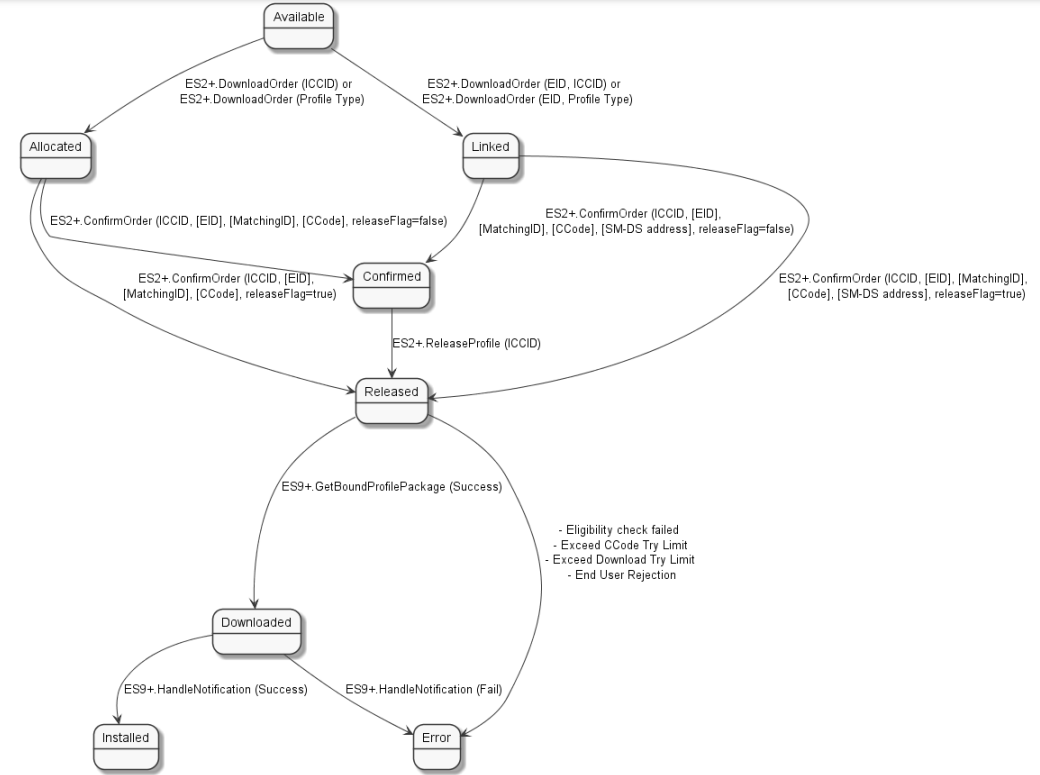
\includegraphics[width=\linewidth]{profile-states1}
\caption{Primo diagramma a stati per i profili eSIM.}
\label{fig:profile-states1}
\end{figure}
\begin{figure}
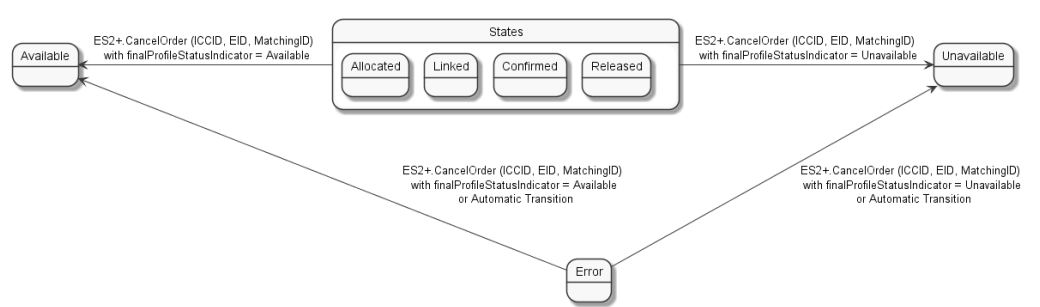
\includegraphics[width=\linewidth]{profile-states2}
\caption{Secondo diagramma a stati per i profili eSIM.}
\label{fig:profile-states2}
\end{figure}
\\Con riferimento alla figura \ref{fig:profile-states1}, a partire dallo stato Available:
\begin{itemize}
\item Si passa allo stato Allocated se si effettua l'ordine di download senza specificare l'EID.
\item Si passa allo stato Linked se si effettua l'ordine di download specificando l'EID.
\end{itemize}
A partire dallo stato Allocated:
\begin{itemize}
\item Si passa allo stato Confirmed se si conferma l'ordine di download con releaseFlag=false.
\item Si passa allo stato Released se si conferma l'ordine di download con releaseFlag=true.
\end{itemize}
A partire dallo stato Linked:
\begin{itemize}
\item Si passa allo stato Confirmed se si conferma l'ordine di download con releaseFlag=false.
\item Si passa allo stato Released se si conferma l'ordine di download con releaseFlag=true.
\end{itemize}
A partire dallo stato Confirmed:
\begin{itemize}
\item Si passa allo stato Released se si effettua il rilascio del profilo in modo tale che sia effettivamente pronto per il download e l'installazione.
\end{itemize}
A partire dallo stato Released:
\begin{itemize}
\item Si passa allo stato Downloaded se il profilo viene consegnato all'LPA con successo.
\item Si passa allo stato Error se si ha un errore nel consegnare il profilo all'LPA.
\end{itemize}
A partire dallo stato Downloaded:
\begin{itemize}
\item Si passa allo stato Installed se il profilo viene installato sull'eUICC con successo.
\item Si passa allo stato Error se si ha un errore nell'installare il profilo sull'eUICC.
\end{itemize}
Con riferimento alla figura \ref{fig:profile-states2}, a partire dagli stati Allocated / Linked / Confirmed / Released:
\begin{itemize}
\item Si torna allo stato Available se l'ordine di download viene annullato con finalProfileStatusIndicator=Available.
\item Si passa allo stato Unavailable se l'ordine di download viene annullato con finalProfileStatusIndicator=Unavailable.
\end{itemize}
A partire dallo stato Error:
\begin{itemize}
\item Si torna allo stato Available in modo automatico oppure se l'ordine di download viene annullato con finalProfileStatusIndicator=Available.
\item Si passa allo stato Unavailable in modo automatico oppure se l'ordine di download viene annullato con finalProfileStatusIndicator=Unavailable.
\end{itemize}

\section{Dettagli su download e installazione dei profili}\label{sec:down-install}
La figura \ref{fig:download-install} ripresa da \cite{GSMA-docs-new} illustra tutti i messaggi che l'operatore, il server SM-DP+, l'LPA e l'eUICC si scambiano tra loro e le operazioni che queste quattro entità svolgono durante la procedura di download e installazione dei profili. Tutti i relativi dettagli \cite{GSMA-docs-new} sono spiegati nelle sottosezioni successive. Anche qui l'intero meccanismo resta valido se si ha un server SM-DS al posto del server SM-DP+, a meno di variazioni di poco conto.
\begin{figure}
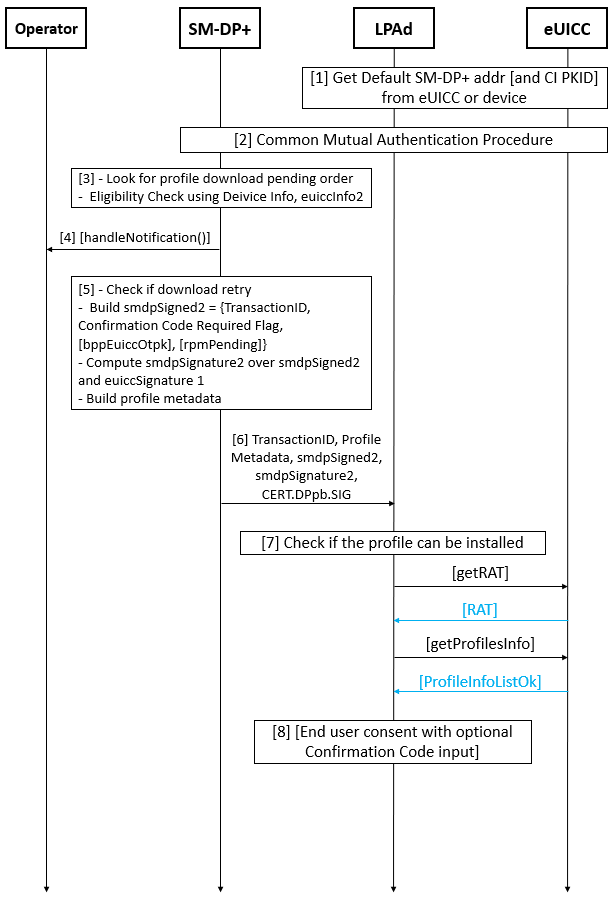
\includegraphics[width=\linewidth]{download-install.png}
\caption{Sequence diagram che descrive il download e l'installazione dei profili.}
\label{fig:download-install}
\end{figure}

\subsection{Condizioni iniziali}
\begin{itemize}
\item L'applicazione LPA potrebbe aver recuperato l'indirizzo del server SM-DP+ e l'identificativo della chiave pubblica del CI Root consentita; se tale identificativo viene effettivamente recuperato a partire dall'eUICC, allora l'LPA deve restringere l'insieme degli identificativi delle chiavi pubbliche dei CI Root compatibili a quel valore.
\item Per ogni profilo nello stato Released il server SM-DP+ mantiene un contatore dei tentativi di download di quel profilo e un contatore dei tentativi di immissione del codice di conferma. Di fatto, il server deve limitare il valore di questi due contatori.
\end{itemize}

\subsection{Procedimento}
\begin{enumerate}
\item Se non lo ha già fatto in precedenza, l'applicazione LPA ottiene l'indirizzo del server SM-DP+ e, opzionalmente, l'OID del server SM-DP+ e l'identificativo della chiave pubblica del CI Root.
\item Viene eseguita la procedura di Common Mutual Authentication definita nella sezione \ref{sec:mutual-auth}.
\item Il server SM-DP+ esegue le seguenti operazioni:
\begin{itemize}[itemsep=0pt]
\item Verificare che esista un'ordinazione di download di un profilo correlato al matching ID, che è l'identificatore della transazione di download corrente.
\item Se l'ordinazione di download del profilo è già linkato a un EID, verificare che quest'ultimo corrisponda all'EID dell'eIUCC appena autenticato.
\item Verificare che il profilo sia nello stato Released o, nel caso di retry a seguito del fallimento di un'installazione precedente, nello stato Downloaded.
\end{itemize}
Se anche solo uno di questi controlli non va a buon fine, la procedura di download e installazione di profili deve essere interrotta. In caso contrario, il server SM-DP+ deve procedere con le seguenti altre azioni:
\begin{itemize}[itemsep=0pt]
\item Incrementare il contatore dei tentativi di download del profilo target. Se il numero massimo di tentativi viene sforato, il server deve notificare l'operatore del fallimento del download e l'intera procedura deve terminare.
\item Effettuare i check di idoneità opportuni.
\end{itemize}
\item Il server SM-DP+ notifica l'operatore con l'esito dei check di validità mediante la funzione \textit{handleNotification} (step opzionale).
\item Se i check di idoneità falliscono, allora il server SM-DP+ esegue le seguenti operazioni:
\begin{itemize}[itemsep=0pt]
\item Portare il profilo target allo stato Error.
\item Restituire uno status di errore all'LPA in modo tale che l'intera procedura termini.
\end{itemize}
In caso contrario, il server SM-DP+ esegue le seguenti altre operazioni:
\begin{itemize}[itemsep=0pt]
\item Determinare se è richiesto un codice di conferma per l'ordinazione pendente.
\item Generare una struttura dati smdpSigned2 che contiene le proprie informazioni.
\item Calcolare smdpSignature2, che è un fingerprint ottenuto da smdpSigned2 ed euiccSignature1, dove euiccSignature1 è un'informazione che è stata scambiata durante la fase di Common Mutual Authetication.
\item Generare i metadati del profilo target.
\end{itemize}
\item Il server SM-DP+ fornisce all'LPA la risposta ad \textit{authenticateClient}, che comprende TransactionID, i metadati del profilo, smdpSigned2, smdpSignature2 e CERT.DPpb.SIG.
\item L'LPA verifica se il profilo può essere effettivamente installato. Per far ciò, deve ricorrere a un'apposita struttura dati detta Rules Authorisation Table (RAT) e/o alla lista dei profili installati. Se non dispone già di queste informazioni, deve richiederle all'eUICC invocando le funzioni \textit{getRAT} e/o \textit{getProfilesInfo}.
\item Se richiesto, l'LPA richiede all'end user di inserire il codice di conferma che l'operatore gli aveva fornito. In caso contrario, l'LPA richiede una conferma semplice (Simple Confirmation) sul download del profilo, che può articolarsi in poche semplici opzioni come 'Yes', 'No', 'Not now'. Se l'end user non inserisce correttamente il codice di conferma o non risponde positivamente alla conferma semplice, si procede con la cancellazione della sessione; altrimenti, l'installazione del profilo può completarsi con successo.
\end{enumerate}

\section{Dettagli sul cambio di dispositivo}
La figura \ref{fig:device-change} ripresa da \cite{GSMA-docs-new} illustra tutti i messaggi che l'end user, l'LPA installata nel vecchio dispositivo, l'eUICC presente nel vecchio dispositivo, il server SM-DP+, l'LPA installata nel nuovo dispositivo, l'eUICC presente nel nuovo dispositivo e l'operatore (qui indicato come Service Provider) si scambiano tra loro e le operazioni che queste sette entità svolgono durante la procedura di trasferimento di un profilo dovuto al cambio di dispositivo. Tutti i relativi dettagli \cite{GSMA-docs-new} sono spiegati nelle sottosezioni successive.
\begin{figure}
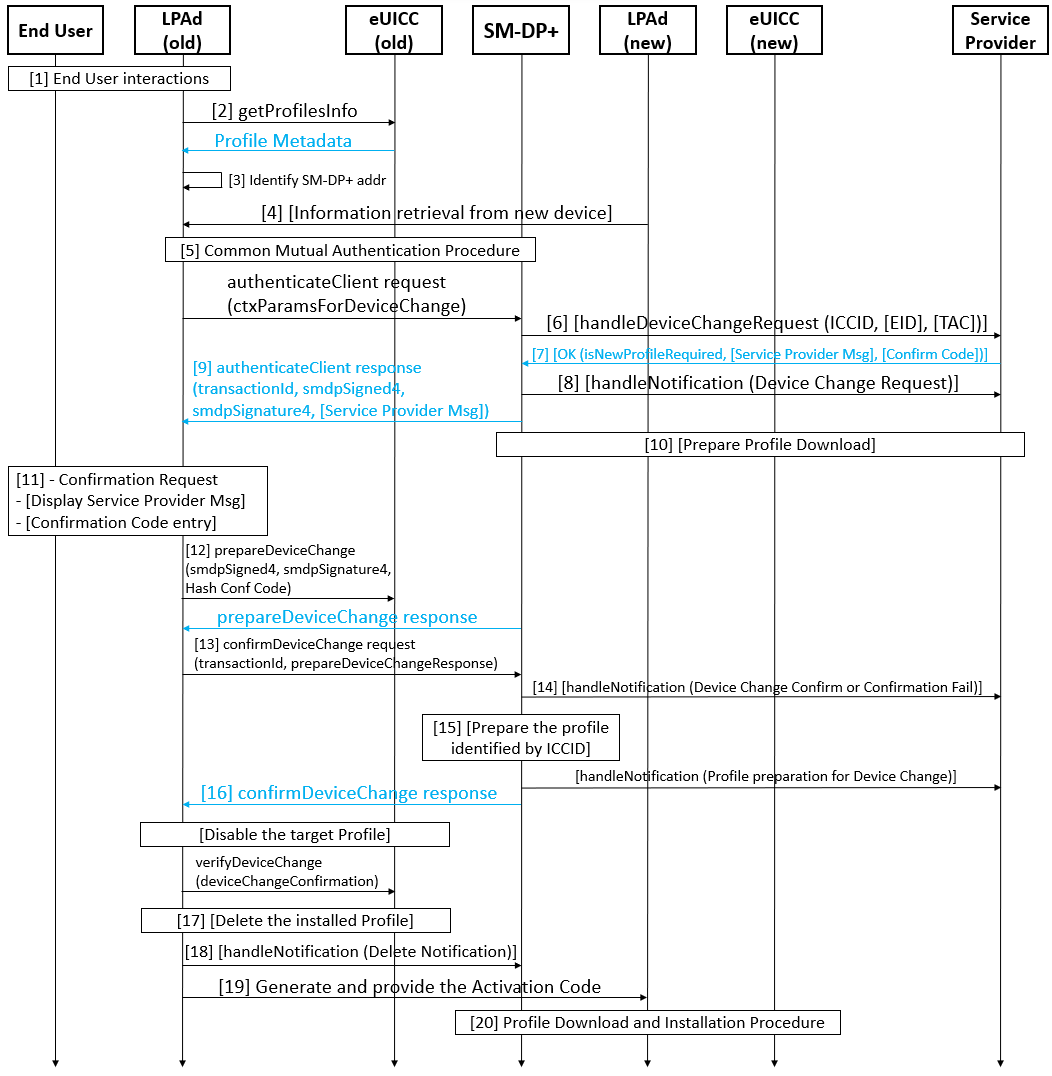
\includegraphics[width=\linewidth]{device-change.png}
\caption{Sequence diagram che descrive il trasferimento di un profilo.}
\label{fig:device-change}
\end{figure}

\subsection{Condizioni iniziali}
\begin{itemize}
\item Il Service Provider ha fornito al server SM-DP+ la configurazione e altre informazioni rilevanti per il cambio di dispositivo. Tutti questi dati devono essere contenuti anche nel profilo all'interno del vecchio dispositivo.
\item L'end user possiede sia un vecchio dispositivo contenente un profilo, sia un nuovo dispositivo.
\item L'eUICC e l'LPA del vecchio dispositivo supportano il cambio di dispositivo.
\end{itemize}

\subsection{Procedimento}
\begin{enumerate}
\item L'end user dà inizio all'operazione di cambio di dispositivo a partire dall'LPA del vecchio dispositivo e seleziona il profilo da installare nel nuovo dispositivo.
\item L'LPA del vecchio dispositivo recupera DeviceChangeConfiguration dai metadati del profilo. Se DeviceChangeConfiguration indica requestToDp, allora si passa allo step (3); se invece DeviceChangeConfiguration indica usingStoredAc, allora si passa allo step (17).
\item L'LPA del vecchio dispositivo determina l'indirizzo del server SM-DP+ a partire da DeviceChangeConfiguration.
\item Se DeviceChangeConfiguration indica che è richiesto l'EID e/o la TAC (Type Allocation Code, che è un codice a 8 cifre univoco per il dispositivo) del nuovo dispositivo, allora l'LPA del vecchio dispositivo recupera l'EID e/o la TAC dal nuovo dispositivo.
\item L'LPA del vecchio dispositivo dà inizio alla procedura di Common Mutual Authentication definita nella sezione \ref{sec:mutual-auth}.
\item Se la funzione \textit{handleDeviceChangeRequest} è configurata nel Service Provider, allora il server SM-DP+ la invoca passandovi come parametri l'ICCID (Integrated Circuit Card ID, che è l'identificativo del profilo) ed eventualmente l'EID e la TAC del nuovo dispositivo. D'altro canto, però, se il server SM-DP+ non supporta il cambio di dispositivo o il cambio di dispositivo non è consentito per il profilo, allora il server risponde con un messaggio di errore e la procedura termina.
\item Il Service Provider risponde al server SM-DP+ col booleano isNewProfileRequired e opzionalmente un messaggio di Service Provider per il cambio di dispositivo e un codice di conferma.
\item Se la funzione \textit{handleNotification} è configurata nel Service Provider, il server SM-DP+ la invoca per notificare il Service Provider riguardo la richiesta del cambio di dispositivo.
\item Il server SM-DP+ restituisce all'LPA del vecchio dispositivo la risposta ad \textit{authenticateClient} che comprende transactionId (l'identificativo della transazione), smdpSigned4 (informazioni del server SM-DP+), smdpSignature4 (signature di smdpSigned4) ed eventualmente il messaggio di Service Provider per il cambio di dispositivo.
\item Se il booleano isNewProfileRequired fornito dal Service Provider nello step (7) vale TRUE, allora il Service Provider esegue il Download Preparation Process (processo di preparazione del download) e opzionalmente il Subscription Activation Process (processo di attivazione della sottoscrizione al profilo).
\item L'LPA del vecchio dispositivo effettua una richiesta di conferma per il cambio di dispositivo. In particolare, se il Service Provider nello step (7) ha fornito il messaggio di Service Provider per il cambio di dispositivo, quest'ultimo viene presentato all'end user. Inoltre, se smdpSigned4 ha il campo ccRequiredFlag pari a TRUE, allora l'LPA del vecchio dispositivo chiede all'end user di inserire il codice di conferma fornito dal Service Provider nello step (7).
\item L'LPA del vecchio dispositivo invoca la funzione \textit{prepareDeviceChange} passandovi come parametri smdpSigned4, smdpSignature4 ed eventualmente l'hash del codice di conferma. Quest'ultimo viene calcolato come SHA256(SHA256(ConfirmationCode) | transactionID).
\item L'LPA del vecchio dispositivo invoca la funzione \textit{confirmDeviceChange} passandovi come parametri transactionID e prepareDeviceChangeResponse.
\item Se il booleano isNewProfileRequired fornito dal Service Provider nello step (7) vale TRUE, allora il server SM-DP+ invoca la funzione \textit{handleNotification} per notificare il Service Provider riguardo l'esito della conferma del cambio di dispositivo da parte dell'end user. Se l'end user ha accettato il cambio di dispositivo, allora si passa allo step (15); altrimenti la procedura termina.
\item Se il booleano isNewProfileRequired vale FALSE, allora il server SM-DP+ prepara il profilo per il download. Inoltre, se nello step (5) è stato fornito un EID, allora il server lo collega col download del profilo preparato. Infine, il server invoca la funzione \textit{handleNotification} per notificare il Service Provider riguardo l'esito della preparazione del profilo.
\item Il server SM-DP+ restituisce all'LPA del vecchio dispositivo la risposta a \textit{confirmDeviceChange} che comprende l'esito del cambio di dispositivo. Se tale risposta contiene encryptedDeviceChangeData, l'LPA del vecchio dispositivo disabilita il profilo target. Dopodiché l'LPA verifica la signature del server SM-DP+ invocando la funzione \textit{verifyDeviceChange}.
\item Se l'esito del cambio di dispositivo lo prevede, l'LPA del vecchio dispositivo deve eliminare il profilo target dall'eUICC del vecchio dispositivo. Inoltre, DeviceChangeConfiguration indica requestToDp e il server SM-DP+ nello step (16) ha indicato di supportare il recovery dei profili eliminati, allora l'LPA del vecchio dispositivo dovrebbe memorizzare alcune informazioni del profilo eliminato, come l'ICCID. Se invece l'eliminazione del profilo non è riciesta, si passa direttamente allo step (19).
\item L'LPA del vecchio dispositivo invia al server SM-DP+ la notifica di eliminazione del profilo. Se l'invio della notifica fallisce, la procedura termina.
\item L'LPA del vecchio dispositivo genera il codice di attivazione (Activation Code) e lo fornisce all'LPA del nuovo dispositivo. Inoltre, dovrebbe fornire al nuovo dispositivo lo stato attuale del profilo in modo tale da consentire all'LPA del nuovo dispositivo di ripristinare correttamente tale stato.
\item Il profilo viene scaricato nel nuovo dispositivo a partire dal server SM-DP+ mediante la procedura di download e installazione dei profili, che è stata definita nella sezione \ref{sec:down-install}.
\end{enumerate}

\chapter{Sicurezza dell'eSIM a run-time}
[TODO]

\chapter{Sicurezza dell'eSIM a boot-time}
\section{Funzionamento del boot dell'eSIM}
[TODO]

\section{Potenziali vulnerabilità}
[TODO]

\section{Prove sperimentali}
[TODO]

\chapter{Conclusione}
[TODO]

\bibliography{Bibliography}

\chapter*{Ringraziamenti}
[TODO]

\end{document}